% !TEX TS-program = lualatex
\documentclass[12pt]{article}
\usepackage{dtj_notas}
\usepackage{sectsty}
\allsectionsfont{\normalfont\sffamily\bfseries}
\usepackage{pgfplots}
\usetikzlibrary{arrows}
\pgfplotsset{samples=300}
\usepackage{ulem}
\newcommand{\UE}[2]{UE_{\text{#1}}(#2)}

\title{\sffamily Notas de Unidad 3\\ \textbf{Juegos estáticos con información incompleta}\\ \normalsize Decisiones y Teoría de Juegos}
\author{Emmanuel Alcalá}
\date{}

\begin{document}
% \setlength{\parskip}{5mm}

\maketitle

\hrule

\begin{summarybox}{Resumen}
	\begin{description}
		\item[Incertidumbre] - Desconocimiento de un jugador sobre el estado del mundo. Se puede modelar de forma probabilística.
		\item[Tipos] - Información que no es de conocimiento común. En ocasiones representada como $ t_i $ o como $ \theta_i $. Los tipos un juego son información privada, y se puede pensar en ellos como una asignación de la Naturaleza (o el azar), que siguen una distribución. Usualmente, la distribución es uniforme. representamos la distribución de los tipos como $ t_i \sim \text{uniforme}(a, b) $.
	\end{description}
\end{summarybox}

\section{Introducción: información}

% c7 de Essentials of game theory, by Leyton-Brown

Los juegos con información completa han asumido que el número de jugadores, las acciones disponibles para los jugadores y los pagos asociados con cada acción son de conocimiento común entre los jugadores.

\begin{summarybox}[colback=red!15]{Nota}
	Información \textbf{incompleta} no es lo mismo que información \textbf{imperfecta}. La información imperfecta es la situación en la que los movimientos de los jugadores no son de conocimiento común (recordar la relación con el conjunto de información).
\end{summarybox}

Si hay información que no es de conocimiento común, entonces hay información \textit{privada}: un agente tiene información sobre sus propias acciones que no saben los otros jugadores. A este fenómeno se le conoce como \textit{información asimétrica}.

El jugador (por ejemplo, A) que desconoce las características de otro jugador (por ejemplo, B) tiene \textit{incertidumbre} sobre las preferencias de dicho jugador. Esto implica que A puede tener conjeturas (creencias) sobre las acciones o los pagos de B. A este conjunto de creencias le llamaremos \textit{tipos}

\begin{exbox}{Ejemplos}
	\begin{myitemize}
		\item Competencia entre empresas que desconocen los costes de sus rivales. Por ejemplo, en el modelo de Cournot, una empresa 2 que recién entra al mercado puede conocer los costes de la empresa 1 y los suyos propios, pero la empresa 1 solo puede darse una idea de los costes de la empresa 2.
		\item Una subasta en la que cada participante conoce su propia valoración del objeto, pero no las de los demás.
		\item Un regateo entre un vendedor y un comprador en la que el primero no conoce la valoración del segundo. Por ejemplo, el comprador ya valuó una casa y sabe su costo: el máximo que está dispuesto a pagar, pero el vendedor no sabe esto.
		\item Un vendedor conoce la verdadera calidad del producto, pero el comprador no. Por ejemplo, la venta de libros usados en Amazon, o la venta de coches seminuevos.
		\item Un trabajador nuevo en la empresa conoce su verdadera productividad y el empresario no.
	\end{myitemize}
\end{exbox}

\subsection*{Subastas (auctions)}

Las subastas son una rama aplicada de la teoría de juegos. Aunque parezcan informales, en realidad tiene una larga tradición de estudio y formalismo matemático, y son usadas por instituciones. Por ejemplo, el Gobierno Federal realiza subastas de bienes improductivos y confiscados por medio del INDEP\footnote{\color{blue}\href{http://subastas.indep.gob.mx/Paginas/Subastas.aspx}{Instituto para Devolverle al Pueblo lo Robado}}.

Las subastas son un \textit{mecanismo} de venta o compra caracterizado por un conjunto de reglas por el que se determina la asignación de recursos y su precio en función de las pujas (oferta) de los participantes. Algunas de sus características benéficas son:

\begin{myitemize}
	\item Eficiencia: se asignan rápidamente a los que la valoran más.
	\item Maximizan los ingresos del vendedor.
	\item Son trasparentes.
\end{myitemize}

Algunas características de la subasta son conocidas (las reglas y la certeza de que se aplicarán, asi como el compromiso del vendedor para no retractarse), pero otras no, como la valoración del objeto a subastar.

Existen varios tipos de subasta, según los mecanismos. Las más comunes son:

\begin{itemize}
	\item \textbf{Inglesa}: el precio se va incrementando sucesivamente hasta que queda un único comprador, el que se adjudica el bien al precio final. Una forma de fijar los precios es que el postor canta su puja (oralmente, mediante un mecanismo electrónico o con un tarjetón a la vista de todos). Mientras superen la puja más alta, pueden ofrecer tantas pujas como deseen.

	\item \textbf{Holandesa}: lo contrario a la anterior. Comienza con un precio muy alto, que va disminuyendo sucesivamente.

	\item \textbf{Sobre cerrado al primer precio}: los postores presentan sus pujas en sobre, el bien se adjudica al mejor postor y el precio es el de la puja más alta. En este caso, \textit{los postores no conocen las pujas de los demás, y cada postor puede presentar una única puja. }

	\item \textbf{Sobre cerrado al segundo precio (subasta de Vickrey)}: igual al anterior, pero el precio del bien no es la puja ganadora, sino la segunda puja más alta.
\end{itemize}

\begin{exbox}{Subasta de dos juadores a sobre cerrado}
	\begin{myitemize}
		\item Dos personas participan en una subasta en sobre cerrado para comprar un cuadro.
		\item Deben elegir \textit{simultáneamente} sus pujas $b_1$ y $b_2$, y el bien se lo adjudica el que haga la puja más alta, pagando lo que ha pujado, y en caso de empatar, se lanza una moneda.
		\item Las \textit{valoraciones} (el valor que las personas le dan al cuadro) son $x_1$ y $x_2$. Las utilidades para el jugador 1 son:
		\[ u_1(b_1, b_2) =
			\begin{cases}
				x_1 - b_1              & \mbox{si } b_1 > b_2 \\
				\frac{1}{2}(x_1 - b_1) & \mbox{si } b_1 = b_2 \\
				0                      & \mbox{si } b_1 < b_2
			\end{cases}
		\]

	\end{myitemize}

	En este caso, hay información \textit{incompleta} porque cada jugador conoce su propia valoración $x_i$ pero desconoce la del rival. Solo sabe, y esto es \textit{conocimiento común}, que cada valoración se ha determinado \textit{ex ante} (antes del cuseo) de forma aleatoria e independiente, por lo que vada valoración tiene una probabilidad asignada, y existe una distribución de probabilidad $\Pr(x_1, x_2)$

\end{exbox}

Una noción importante es que este tipo de juegos es considerar que el movimiento \textit{ex ante} lo ha realizado la Naturaleza, que con cierta probabilidad asigna un \textit{tipo} de juego (por ejemplo, un tipo $x_1$ o $x_2$). El siguiente ejemplo lo dejará más claro.

\subsection*{Juego de entrante e incumbente}

\begin{figure}[H]
	\centering
	\footnotesize{Second
		\begin{forest} decision tree,for tree={s sep=25pt}
				[E1, plain content
						[{0, 2};Salir,plain content,elo={yshift=4pt}]
						[E2;Entrar,plain content,elo={yshift=4pt}
								[{-1,-1};Pelear]
								[{1,1};Acomodar]
						]
				]
		\end{forest}}
	\caption{Juego de entrada simple}
	% \label{fig:fig6}
\end{figure}

Considerar ahora que existe un jugador 1 y dos \textit{tipos} de jugador 2, y el jugador 1 podría jugar con cualquiera de ellos. El primer tipo de jugador 2 obtiene las mismas ganancias, pero el segundo tipo, un jugador loco, disfruta pelear y obtendría 2 en vez de -1 si juega (Entrar, Pelear).

\begin{figure}[H]
	\centering
	\footnotesize{
		\begin{forest} decision tree,for tree={s sep=25pt}
			[Naturaleza, plain content
			[E1;p,plain content,elo={yshift=4pt},alias=e1i
			[{0, 2};S,plain content,elo={yshift=4pt}]
			[E2;En,plain content,elo={yshift=4pt}
				[{-1,-1};P]
				[{1,1};A]
			]
			]
			[E1;1-p,plain content,elo={yshift=4pt},alias=e1d
			[{0, 2};S,plain content,elo={yshift=4pt}]
			[E2;En,plain content,elo={yshift=4pt}
				[{-1,2};P]
				[{1,1};A]
			]
			]
			]
			\draw[dashed,transform canvas={yshift=-6pt}] (e1i) to[right=45] (e1d);
		\end{forest}}
	\caption{Juego de entrada con información incompleta.}
	% \label{fig:fig6}
\end{figure}

En el segundo juego, conceptualizamos a un nuevo jugador Naturaleza que elige con qué tipo de jugador 2 va a jugar el jugador 1, con una probabilidad $p, 1-p$. La estructura del juego no cambia mucho, dado que existen $i=1,...,N$ jugadores con las mismas acciones $A_i$.

Asumimos, además, que $p$ representa una creencia del jugador 1 sobre los tipos del jugador 2. A esto se le conoce como \textit{la asunción a priori común}. Significa que todos los jugadores están de acuerdo en que la Naturaleza escoja con cuerta probabilidad los diferentes tipos de jugadores.



\textbf{En resumen:}
\begin{myitemize}
	\item Por \textit{tipos} nos referiremos a cualquier información que describa por completo \textit{la información que no es de conocimiento común}, sino privada.
	\item Cada jugador conoce su propio \textit{tipo} con certidumbre completa.
	\item Las creencias de un jugador sobre los \textit{tipos} de otros jugadores son capturadas por una distribución de probabilidad conjunta sobre esos tipos, y esta distribución es de \textit{conocimiento común}.
	\item Los tipos pueden representarse como \textit{tipos de juego}.
	\item Un jugador, Naturaleza, \textit{decide} qué tipo de juego se juega.
	\item La incertidumbre sobre tipos es descrita como la Naturaleza escogiendo tipos \textit{para} los jugadores.
	\item Dado que la incertidumbre sobre los tipos son conjeturas (o creencias) que se modelan como una distribución de probabilidad \textit{a priori} (o anterior), esta distribución es de conocimiento común. Es decir, es de \textit{conocimiento común} cómo la Naturaleza escoge los tipos para los jugadores.
\end{myitemize}

Por ejemplo, en un juego de Cournot, E1 puede no saber el costo de producción de E2, $C_2(q_2)$, pero puede conjeturar que sus costos marginales (constantes) pueden ser altos o bajos, $c_A$ y $c_B$, en cuyo caso podría ser $C_2(q_2)=c_Aq_2$ o $C_2(q_2)=c_Bq_2$.

E1 tiene un solo tipo,  $T_1 = \{c\}$, mientras que E2 tiene dos tipos, $T_2 = \{c_A, c_B\}$. Dado que el costo de E2 \textit{impone} restricciones sobre el juego que jugará E1 (dado que la Naturaleza escoge el tipo que habrán de jugar), existe cierta dependencia entre ambos. Si es de conocimiento común la distribución sobre los tipos $p(t)$, E1 podría resolver su incertidumbre formándose una conjetura.

En particular, si E1 conjetura que el costo de E2 depende del de E1, podría usar esa información condicionando el tipo de E2 a su tipo, $p(c_A|c), p(c_B|c)$. Ya que tiene una forma de tratar sus creencias sobre los tipos (costos) de E2, podría evaluar sus estrategias puras $S_i$, o, para simplificarlo, dado que se trata de estrategias puras, usaremos $A_i$, por ejemplo, $a_1$ sería la cantidad $q_1$. La función de ganancias de E1 será $u_1(q_1, q_2;c) = [a - (q_1 + q_2) - c]q_1$, pero en este caso, E2 tendrá dos funciones de ganancia:

\begin{align*}
	u_2(q_1, q_2;c_A) =  [a - (q_1 + q_2) - c_A]q_2 \\
	u_2(q_1, q_2;c_B) =  [a - (q_1 + q_2) - c_B]q_2
\end{align*}

Aún nos falta cómo se obtiene un EN en este caso, dado que E1 debe escoger una BR para la BR de E2, que puede depender de $c_A$ o $c_B$ \footnote{Este juego se resuelve más adelante.}.

\subsection{Forma normal de un juego bayesiano}

\begin{summarybox}[colback=red!15]{Nomenclatura}

	Para todo jugador $i \in N$:

	\begin{myitemize}
		\item $T_i$: el conjunto o espacio de tipos del jugador $i$. Tadelis usa una nomenclatura diferente para los tipos, $\Theta \text{ en vez de } T$.
		\item $t_{i1}, t_{i2}, ..., t_{ik}$: $k$ tipos del jugador $i$, con $t_{i} \in T_i$. En Tadelis, $t_{i}$ es $\theta_{i}$.
		\item $T_{-i}$ y por extensión $t_{-i}$: son los tipos de los jugadores no-\textit{i}. En Tadelis es $\Theta_{-i}, \theta_{-i}$.
		\item $p(t_{-i}|t_i)$: probabilidad condicional que representa la conjetura que el jugador $i$ tiene sobre el tipo del jugador $-i$. Es decir, es la conjetura que $i$ tiene sobre los tipos $t_{-i}$ de los otros jugadores, \textit{dado} su conocimiento sobre su propio tipo $t_i$. Lo que el jugador $i$ sabe es $t_i$, y lo que desconoce es $t_{-i}$, y la $p(\cdot, \cdot)$ es la \textit{asignación} de credibilidad a las posibilidades, que se resolverá con el teorema de Bayes más adelante. En Tadelis, $p_i$ se denota con $\phi_i$
		\item $A_i$: espacio de acción del jugador $A_i$.
	\end{myitemize}
\end{summarybox}

\begin{mybox}{Definición: Forma normal de un juego bayesiano}
	\begin{defi}
		La representación normal de un juego Bayesiano de información incompleta con $n$-jugadores es:
		\[ \langle N, \{A_i \}_{i=1}^n, \{ T_i \}_{i=1}^n, \{u_i(\cdot; t_i ), t_i \in T_i\}_{i=1}^n, \{ p_i \}_{i=1}^n \rangle \]

		Para los espacios $A_1, A_2, ..., A_n$, con $a_{i1}, a_{i2}, ..., a_{ik} \in A_i$; los espacios de los \textit{tipos} por jugador $T_1, ..., T_n$ con $t_{i1}, t_{i2}, ..., t_{ik} \in T_i$; para un tipo de jugador $i$, $t_i$, conocido solo por el jugador $i$, determina la función de ganancia $u_{i}(a_1, a_2, ..., a_n; t_i)$; la conjetura de $i$ sobre los tipos $t_{-i}$, $p_i(t_{-i}|t_i)$ describe la incertidumbre de $i$ respecto a los posibles tipos de los $n-1$ jugadores, dado el tipo de $i$.

	\end{defi}
\end{mybox}

En el duopolio de Cournot, $N = \{1, 2\}$, $A=\{q_1, q_2 \}$,  con, por ejemplo,  $a_2 = q_2$, $T = \{\{c\}, \{c_A, c_B\}\}$, con, por ejemplo, $t_{21} = c_A$; la función de ganancias $u_i(q_1, q_2; t_i)$, por ejemplo $u_1(q_1, q_2; c)$; y finalmente, $p_i(t_{-1}|t_i)$, con por ejemplo, $p_1(c_B|c)$ la conjetura o creencia de E1 con respecto al tipo $c_B$ condicionado sobre su costo.

\begin{summarybox}[colback=red!15]{Nota}
	En la mayoría de los juegos analizados, los tipos son independientes, por lo que $p_i(t_{-1}|t_i) = p_i(t_{-i})$. Es decir, la creencia del jugador $i$ sobre el tipo de otro jugador, condicionada a su propio tipo $t_i$, es simplemente la probabilidad del tipo del jugador $-i$. Los casos en los que esto no sucede son los juegos donde las estrategias de los jugadores están correlacionadas, pero no los analizaremos.
\end{summarybox}

\subsubsection{Desarrollo temporal de un juego bayesiano}

Una vez que introducimos al \textit{jugador} Naturaleza, podemos suponer que el juego se desarrolla de la siguiente forma:

\begin{myenum}
	\item La Naturaleza (= azar) determina un vector de tipos $t = (t_1,...,t_n)$, que se obtiene a partir de un conjunto de tipos \textit{posibles} $T_i$.
	\item Se revela el tipo $t_i$ al jugador $i$, pero a ningún otro jugador.
	\item Los jugadores toman sus decisiones de forma \textit{simultánea}; $i$ elige $a_i$ de $A_i$.
	\item Se reciben las ganancias $u_i(a_1,...,a_n;t_i)$.
\end{myenum}

Es importante señalar: la introducción de Naturaleza como otro jugador convierte un juego con información \textit{incompleta} en un juego con información \textit{imperfecta}.

Esto es así porque en una etapa del juego, al jugador que le corresponde decidir \textit{desconoce} el desarrollo del juego previo la etapa. Dado que la Naturaleza revela el tipo de juego al jugador $i$, pero no al jugador $j$, $j$ no conoce la historia completa del juego cuando toma su decisión en el paso \textbf{3}.

Aún falta algo. Dada la creencia \textit{a priori} sobre la distribución de los tipos, $p(t)$, ¿cómo resolvemos la conjetura de $i$, $p_i(t_{-i}|t_i)$?

Con el \textbf{teorema de Bayes}:

\[ p_i(t_{-i}|t_i) = \frac{p(t_{-i}, t_i)}{p(t_i)} \]

% \subsubsection{Teorema de Bayes}

% Sea ${ B}_1, { B}_2, { B}_3, ... { B}_n$ una \emph{partición} del espacio muestral (i.e., son disjuntos y su unión es el espacio muestral entero).

% \begin{align*} 
% P({ A}) &= P({ A} | { B}_1)P({ B}_1) + P({ A} | { B}_2)P({ B}_2) + \dots + P({ A} | { B}_n)P({ B}_n)\\
% P({ A}) &= P({ A} \cap { B}_1)+ P({ A} \cap { B}_2)+ \dots + P({ A} \cap { B}_n)
% \end{align*} 

% Como se puede ver en la siguiente figura, la totalidad de $A$ se obtiene con la unión de la intersección de $A$ con $B$. Es decir, 

% \[A=\bigcup^n_{i=1}(A \cap B_i)\]

% \begin{figure}[H]
%     \centering
%     	\includegraphics[scale=0.7]{particion}
%     \caption{Partición de A en 4}
%     % \label{fig:my_label}
% \end{figure}

% Suponiendo que $n=4$, por lo tanto, la probabilidad de $A$ se obtiene con la probabilidad de la unión de la intersección de $A$ con $B$, es decir.

% \begin{equation}
%     P(A)=\sum_{i=1}^{4}P(A \cap B_i)
%     \label{eq:p_total}
% \end{equation}

% A la ecuación \ref{eq:p_total} se le conoce como \textit{Ley de probabilidad total}.

% Si $A$ y $B$ ocurren conjuntamente, su probabilidad se puede obtener como

% \begin{align*} 
% P(A,B) &= P(A)P(B|A) \\
% P(A,B) &= P(B)P(A|B)
% \end{align*}

% Igualando la parte derecha de ambas ecuaciones, nos lleva al teorema de Bayes

% \begin{align}
%     P(A)P(B|A) = P(B)P(A|B) \\
%     P(B|A)     = \frac{P(B)P(A|B)}{P(A)}
%     \label{eq:teo_bayes}
% \end{align}

% En la ecuación \ref{eq:teo_bayes}, a la cantidad $P(B|A)$ se le conoce como probabilidad (o distribución) posterior, que es \textit{desconocida } antes de que $A, B$ y $A,B$ (conjuntamente) ocurran. Todas las probabilidades de la derecha son, en cierto sentido, \textit{a priori}, aunque en el contexto de la estadística tienen otros nombres y solo $P(A)$ es considerada \textit{a priori}. 

\subsection{Equilibrio de Nash Bayesiano, ENB}

\begin{mybox}{Definición (estrategias en juegos bayesianos)}
	\begin{defi}
		En un juego bayesiano estático, una estrategia del jugador $i$ es una función $s_i(t_i)$ donde, para cada tipo $t_i \in T_i$, la función $s_i(t_i)$ \textit{determina} la acción del conjunto $A_i$ que \textbf{sería} elegida si la Naturaleza \textit{decide} que el jugador $i$ será de tipo $t_i$.
		Es decir:

		\[s_i\colon t_i \mapsto A_i \]

	\end{defi}
\end{mybox}

Nótese que la estrategia no forma parte de la representación normal, a diferencia de los juegos con información completa. La estrategia se determina \textit{a partir} de los tipos y acciones diponibles. Por ejemplo, en el duopolio de Cournot que hemos descrito, E1, aunque solo tiene un tipo-costo $c$, deberá elegir una $q_1$ \textit{por cada} costo-tipo de E2, de tal forma que pueda determinar si la cantidad $q_1^*$ constituye en efecto su BR a E2.

En el juego de entrada, si los dos tipos del jugador E2 son $t_2 = (racional, loco)$, las acciones de E2 serán

\begin{figure}[H]
	\centering
	\footnotesize{
		\begin{forest} decision tree,for tree={s sep=25pt}
			[Naturaleza, plain content
			[E1;p,plain content,elo={yshift=4pt},alias=e1i
			[{0, 2};S,plain content,elo={yshift=4pt}]
			[E2;En,plain content,elo={yshift=4pt}
				[{-1,-1};P]
				[{1,1};A]
			]
			]
			[E1;1-p,plain content,elo={yshift=4pt},alias=e1d
			[{0, 2};S,plain content,elo={yshift=4pt}]
			[E2;En,plain content,elo={yshift=4pt}
				[{-1,2};P]
				[{1,1};A]
			]
			]
			]
			\draw[dashed,transform canvas={yshift=-6pt}] (e1i) to[right=45] (e1d);
		\end{forest}}
	\caption{Juego de entrada con información incompleta.}
	% \label{fig:fig6}
\end{figure}

\begin{align*}
	s_2(t_2) =
	\begin{cases}
		Pelear \text{ si } t_2 = loco \\
		Acomodar \text{ si } t_2 = racional
	\end{cases}
\end{align*}


La noción de ENB es una idea simple: la estrategia de cada jugador debe ser una MR (mejor respuesta) a las estrategias de los restantes jugadores (que, de nuevo, dependerán del tipo que sea seleccionado por Naturaleza). El ENB es un equilibrio de Nash en un juego bayesiano. Un juego bayesiano es aquel donde la incertidumbre respecto de los tipos se representa como una distribución de probabilidad sobre los posibles tipos. Un tipo posible es aquel cuyo soporte es positivo, $p_i(t_{-i})>0$.

\begin{mybox}{Equilibrio de Nash Bayesiano}
	\begin{defi}
		En el juego bayesiano estático,

		\[ \langle N, \{A_i \}_{i=1}^n, \{ T_i \}_{i=1}^n, \{u_i(\cdot; t_i ), t_i \in T_i\}_{i=1}^n, \{ p_i \}_{i=1}^n \rangle \]

		las estrategias $s^* = (s_1^*, s_2^*, ..., s_n^*)$ forman un equilibrio de Nash bayesiano (\textbf{ENB}) \textit{en estrategias puras} si, para cada jugador $i$ y para cada uno de sus tipos $t_i$, la función de estrategia $s_i^*(t_i)$ es una solución de

		\[ \sum_{t_{-i} \in T_{-i}} u_i(s_i^*(t_i), s_{-i}(t_{-i}); t_i)p(t_{-i} | t_i) \geq
			\sum_{t_{-i} \in T_{-i}} u_i(a_i, s_{-i}(t_{-i}); t_i)p(t_{-i} | t_i)
		\]

		Recordar que la estrategia mapea un tipo a una acción, es decir, $s(t) = a$. Por $a_i$ nos referimos a cualquier {\color{blue}$a$} \textit{que no sea} resultado de $s_{i}^*(t_i)$.

		La expresión anterior se puede expresar altenativamente como:

		\[\max \sum_{t_{-i} \in T_{-i}} u_i(s_i(t_i), s_{t_{-i}}^*; t_i)p(t_{-i} | t_i) \]

	\end{defi}
\end{mybox}

\begin{summarybox}[colback=red!15]{Nota}
	Recordar la definición de valor esperado

	\[
		\textbf{E}[X] = \sum_i p_i x_i
	\]
	Por lo que
	\[ \sum_{t_{-i} \in T_{-i}} u_i(s_i^*(t_i), s_{-i}(t_{-i}); t_i)p(t_{-i} | t_i) \]
	es se puede escribir como

	\[
		\textbf{E}[u_i(s_i^*(t_i), s_{-i}(t_{-i}); t_i)]
	\]

	Que es el valor esperado de la utilidad del jugador $i$. El problema se convierte entonces en

	\[
		\max_{t_{-i}} \textbf{E}[u_i(s_i^*(t_i), s_{-i}(t_{-i}); t_i)]
	\]

\end{summarybox}

\section{Ejemplos}

\begin{exbox}{NoC bayesiano}
	Suponer que Ale y Fer conocen sus propias ganancias, pero desconocen las de la otra, que podrían ser ligeramente mayores a 2. $t_A$ define el tipo de Ale, y $t_F$ el de Fer.

	\begin{center}
		\begin{game}{2}{2}[Fer][Ale]
			&      N         &   C     \\
			N  &  2+$t_F$, 1    &  0,0    \\
			C  &   0,0          &  1, 2+$t_A$
		\end{game}
	\end{center}

	La naturaleza asigna $t_A$ a Ale y $t_F$ a fer, de modo que las ganancias de cada una por su actividad preferida son ligeramente mayores que dos si $t_i > 0$. Para continuar con el ejemplo, asumamos que $t_A, t_F \sim \text{Unif}(0, 2)$, que $t_A, t_F $ solo afectan a las ganancias.

	El juego se puede representar como

	\[J=\{ Ale, Fer, A_A, A_F; T_A, T_F; p(t_A), p(t_F); u_A, u_F  \} \]

	Con $A_A=A_F=\{N, C \}$, y $T_A, T_F \in (0, 2)$. No usaremos un árbol, porque son espacios de decisión continuos. Ahora, ¿cómo podemos resolverlo? Las jugadoras podrian usar la siguiente estrategia

	\[
		s_F(t_F) = \begin{cases}
			N \text{ si } t_F \geq k \\
			C \text{ si } t_F < k
		\end{cases}
	\]

	Lo mismo para Ale

	\[
		s_A(t_A) = \begin{cases}
			N \text{ si } t_A \geq l \\
			C \text{ si } t_A < l
		\end{cases}
	\]

	Es decir, si su tipo es mayor a un valor $k\in (0, 2)$, cada jugadora eligirá su actividad favorita. ¿Con qué probailidad eligirán dicha actividad? La función de densidad de $x \sim \text{uniforme}(a, b)$ es

	\[ p(x) = \frac{1}{b-a} \]

	Para encontrar la probabilidad deseada, debemos integrar $p(x)$ entre $[\theta, 2]$, que se logra con

	\begin{align*}
		p(t_i \geq \theta) & = 1 - p(t_i < \theta)                                 \\
		                   & = 1 - \int_0^\theta \frac{1}{2} dx                    \\
		                   & = 1 - \Bigg[ \frac{x}{2} \Bigg]_0^\theta              \\
		                   & = 1 - \frac{1}{2} (\theta - 0) = 1 - \frac{\theta}{2}
	\end{align*}

	para $\theta=\{k, l\}$.

	Existe otra forma más sencilla para calcular. Dado que la distribución uniforme se puede describir como un rectángulo

	\begin{center}
		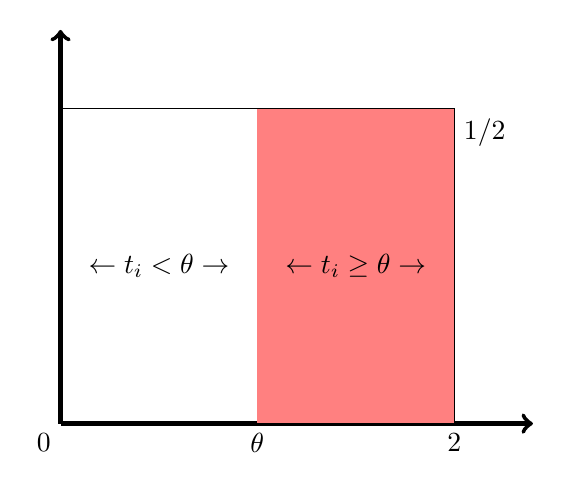
\begin{tikzpicture}
			\draw[->,ultra thick] (0,0)--(6,0);
			\draw[->,ultra thick] (0,0)--(0,5);
			\fill[red!50]    (2.5,0) rectangle  ++ (2.5,4) node[below right] {\color{black}$1/2$} ;
			\draw            (0,0) node[below left] {0} rectangle  ++ (5,4);
			\draw (5, 0) node[below] {2} (2.5, 0) node[below] {$\theta$};
			\draw (2.5+2.5/2,2) node {$\leftarrow t_i \geq \theta \rightarrow$};
			\draw (2.5/2,2) node {$\leftarrow t_i < \theta \rightarrow$};
		\end{tikzpicture}
	\end{center}

	El área de la zona en rojo es

	\[ \underbrace{(2-\theta)}_{\text{base}} \times \underbrace{ \frac{1}{2}}_{\text{altura}} \]

	$\frac{2-k}{2}$

	El problema se resuelve como ya sabemos

	\begin{center}
		\begin{game}{3}{3}[Fer][Ale]
			&      N         &   C         &   \\
			N  &  2+$t_F$, 1    &  0,0        & $1 - k/2$  \\
			C  &   0,0          &  1, 2+$t_A$ & $1-(1-k/2)=k/2$ \\
			&  $l/2$    &    $1-l/2$ & \\
		\end{game}
	\end{center}


	\begin{align*}
		UE_{Fer}(N) & = \frac{l}{2}\Bigg(2+t_F\Bigg) + \Bigg(1-\frac{1}{2}\Bigg)0=\frac{l}{2}(2+t_F) \\
		UE_{Fer}(C) & = \frac{l}{2}0 + \Bigg(1-\frac{1}{2}\Bigg)1=1-\frac{1}{2}
	\end{align*}

	Sabemos que no es óptimo para Fer si $UE_{Fer} \geq UE_{Fer}(C)$

	De lo cual resulta $t_F \geq \frac{2}{l}-3$. Dato que nos preguntamos $t_F\geq k$ entonces $\frac{2}{l}-3= k$.

	Para Ale resulta algo similar, en donde $UE_{Ale}(C)\geq UE_{Ale}(N)$, con resultado de $t_{A}\frac{2}{k}-3=l$.

	Debemos resolver el sistema

	\begin{align*}
		t_{F} & \geq k = \frac{2}{l}-3 \\
		t_A   & \geq l = \frac{2}{k}-3
	\end{align*}

	Resolviendo esto nos da

	\[
		\theta^2 + 3\theta - 2=0\quad \text{para } \theta=(l, k)
	\]

	Que se resuelve con la fórmula general para ecuaciones cuadráticas, par $ax^2 + bx + c$

	\[
		\frac{-b \pm \sqrt{b^2 - 4ac}}{2a}
	\]

	La probabilidad de que Fer elija N era $p_F(t_F\geq k) = 1 - \frac{1}{2}k$, por lo tanto

	\[
		1 - \frac{1}{2} \Bigg(\frac{-3 + \sqrt{9 - 4(1)(-2)}}{2}\Bigg) = 0.72
	\]

	Lo mismo para Ale.

	(Solo sumamos la raíz, dado que su resta daría una probabilidad negativa).

	Suponer ahora que $t_A, t_F \in [0, x]$, ¿qué pasa conforme $x \rightarrow 0$?

	Se tiene que resolver

	\[
		\lim_{x\rightarrow 0} \Bigg [ 1 - \Bigg ( \frac{-3+\sqrt{9+4x}}{2x} \Bigg) \Bigg ]
	\]

	Usando regla de L'Hopital

	\[
		\lim_{x\rightarrow c} \frac{f(x)}{g(x)} = \lim_{x\rightarrow c} \frac{f'(x)}{g'(x)}
	\]

	Para $f(x)$

	\[
		\frac{d(\sqrt{9+4x} - 3)}{dx} = \frac{2}{\sqrt{9+4x}}
	\]

	Para $g(x)$

	\[
		\frac{d(2x)}{dx} = 2
	\]

	Aplicando regla de L'Hopital

	\[
		\lim_{x\rightarrow 0} \frac{f'(x)}{g'(x)} = \frac{\frac{2}{\sqrt{9+4x}}}{2} = \frac{2}{2 \sqrt{9+4x}}=\frac{1}{3}
	\]

	¿Cuál es el resultado de un juego con información completa, pero con estrategias mixtas, para el juego de NoC?

	\begin{center}
		\begin{game}{2}{2}[Fer][Ale]
			&      N     &   C\\
			Netflix   & $2,1$  & $0,0$\\
			Café      & $0,0$  & $1,2$
		\end{game}
	\end{center}

	Cuando se elimina la información incompleta (la incertidumbre), el resultado es el de estrategias mixtas.

\end{exbox}

\begin{exbox}{Subasta de sobre cerrado a la primera puja}

	Dos jugadores pujan por una pintura. La pintura se la gana el jugador con la mayor puja, con un precio al costo de su puja.

	Por ejemplo, si J1 puja 290 y J2 310, J2 gana y paga por la pintura 310.

	Si J2 valúa en $x_2$ la pintura, su ganancia sería $x_2 - 310$, y la de J1 sería 0. En general

	\[
		u_i(b_i, b_j)=\begin{cases}
			x_i - b_i\quad & \text{ si } b_i > b_j \\
			0 \quad        & \text{ si } b_i < b_j
		\end{cases}
	\]

	Supongamos que el jugador $i$ puja una fracción $a$ de su valuación $x_i$, es decir $b_i = ax_i$. Suponer que $j$ también ofrece $b_i = a x_j$, y dado que es la misma $a$, la estrategia es simétrica.

	Para simplificar un poco la notación, supongamos que la puja de $i$ es $y$. El jugador $i$ gana si y solo si la puja de $j$ es menor que $y$, es decir $b_i<y$ o $ab_j<y$.

	Asumir que
	$$
		x_i \sim \text{uniform}(0, 100)
	$$

	y la puja de ambos jugadores $b_i \in [0, x_i], i= \{1, 2\}$.

	¿Cuál es el ENB $(b_1, b_2)$? (simétrico).

	Sol.

	El jugador $j$ puja $b_i = ax_j$, $i$ puja $y$. Necesitamos la utilidad esperada, y maximizar esta utilidad. Maximizar $\textbf{E}[u_i(s_i^*(t_i), s_{-i}(t_{-i}); t_i)]$

	\[
		UE_i(y, b_j) = \underbrace{x_i-y}_{u_i\text{ si gana }} \times p(\text{gana}) + \underbrace{0}_{u_i\text{si pierde}} p(\text{perder})
	\]

	¿Cuál es la probabilidad de ganar? el jugador $i$ gana si $y>b_j$, es decir si $y>ax_j$. Dicho de otra forma, el jugador $i$ debe ofrecer $x_j < y/a$, y la probabilidad de que esto suceda es

	\[
		p(x_j < y/a) = \int_0^{y/a} \frac{1}{100}dw = \Bigg[\frac{w}{100} \Bigg]_0^{y/a} = \frac{y}{100a} \]

	\begin{center}
		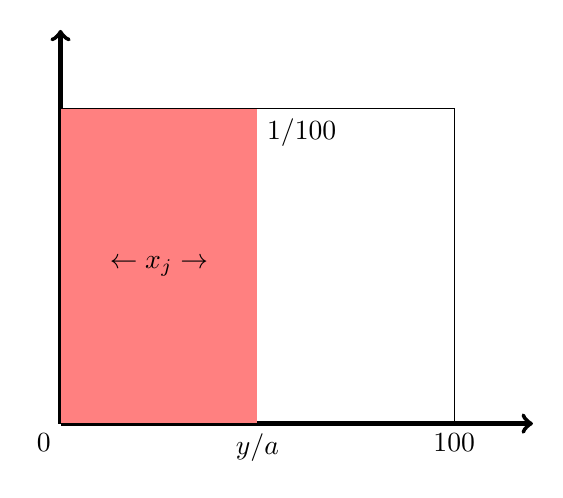
\begin{tikzpicture}
			\draw[->,ultra thick] (0,0)--(6,0);
			\draw[->,ultra thick] (0,0)--(0,5);
			\fill[red!50]    (0,0) rectangle  ++ (2.5,4) node[below right] {\color{black}$1/100$} ;
			\draw         (0,0) node[below left] {0} rectangle  ++ (5,4);
			\draw (5, 0) node[below] {$100$} (2.5, 0) node[below] {$y/a$};
			\draw (2.5/2,2) node {$\leftarrow x_j \rightarrow$};
		\end{tikzpicture}
	\end{center}

	La probabilidad de ganar entonces es

	\begin{align*}
		UE_i(y, b_j) & =p(\text{gana})(x_i - y)                          \\
		             & =\frac{y}{100a}(x_i - y)=\frac{x_i y - y^2}{100a}
	\end{align*}

	Recordar cómo obtenemos el ENB:

	\[\max \sum_{t_{-i} \in T_{-i}} u_i(s_i(t_i), s_{t_{-i}}^*; t_i)p(t_{-i} | t_i) \]

	Que se convierte en este problema en

	\[\max \sum_{b_j \in B} u_i(y, b_j; b_i)p_i(b_j) = \max_{y} UE_i(y) = \max_y \frac{x_i y - y^2}{100a} \]

	O alternativamente

	\[ y^* = \argmax_{0<y<x_i} \frac{x_i y - y^2}{100a} \]

	Que se resuelve con condiciones de primer orden

	CPO:

	\[
		\frac{\partial UE_i}{\partial y} = 0 \Longrightarrow \frac{x_i - 2y}{100a}
	\]

	Nota:

	\[
		\frac{\partial}{\partial y}\frac{x_i y - y^2}{100a} = \frac{1}{100a}\frac{\partial}{\partial y}(x_iy - y^2)=\frac{1}{100a}(x_i - 2y)=0
	\]

	Eliminamos $1/100a$, por lo tanto

	\[
		x_i - 2y = 0 \Longrightarrow y = \frac{1}{2}x_i
	\]

	Dado que el jugador $i$ ofrece $y=ax_i$, concluimos que $a = 1/2$. El juego claramente lo va a ganar alguien que valore más.

	Por ejemplo, si $x_1 = 200, x_2 = 300$, entonces $b_1 = (1/2)200 = 100, b_2 = (1/2)300 = 150$ y $b_1 < b_2$.

\end{exbox}

\subsection{Información asimétrica}

\begin{mybox}[colback=red!30, coltitle=black]{Nota}
	\textit{Cita adaptada de Tadelis, p. 258}

	Una de las mayores concluisiones del análisis de mercados competitivos es que los mercados distribuyen bienes a los agentes que más los valoran. Si un bien es mal asignado, de tal manera que lo obtiene una persona que que lo valúa menos que otra, las ``presiones del mercado'' causarán que el precio del bien incremente a un nivel que los poseedores actuales preferirán venderlo que quedárselo (es decir, si su valuación es $v_1$ y la valuación de un potencial comprador es $v_2$ con $v_2 > v_1$ tendrían una potencial ganancia $v_2 - v_1$), y la gente que lo valore más estará dispuesta a comprarlo. Mecanismos como negociación, subastas o el mercado de intermediarios podrían ayudar a fijar el precio.

	El anterior argumento está basado en algunas asunciones. Por ejemplo, que el valor del bien es conocido y entendido por todos los participantes, es decir, existe \textit{información perfecta} sobre el valor  del bien.

\end{mybox}

Cuando existe información asimétrica (un jugador mejor información sobre la cualidad de un bien) pueden suceder efectos de \textit{selección adversa}. Esta situación sucede cuando una de las partes no es capaz de decidir la calidad de un producto o servicio ofrecido por la otra parte.

El término surgió originalmente en las agencias de seguros, en donde las personas propensas a contratar seguros normalmente son las más expuestas a riesgos. Por ejemplo, en una población $P$ con una fracción de fumadores $\alpha, 0 < \alpha < 1$, y una fracción de no fumadores $1-\alpha$. Si la aseguradora no puede distinguir entre ambos (en donde el cliente no fumador es de 'mejor' calidad), en una selección adversa la aseguradora puede terminar asegurando $\alpha P > (1-\alpha)P$, dedibo a que los no fumadores podrían considerar que al comprar el seguro subsidian a los fumadores.


\begin{exbox}{Mercado de coches usados (The Market for Lemons)}

	En el mercado de coches usados existe información asimétrica

	\begin{myitemize}
		\item El vendedor conoce mucho mejor la calidad del producto. Por ejemplo, si ha tenido accidentes y reparaciones. El comprador no necesariamente conoce esto, ni puede acceder a esa información antes de la compra.
		\item Existe un incentivo para que el vendedor pase productos de baja calidad por productos de alta calidad.
		\item Existen deficiencias de seguridades públicas efectivas que vigile la calidad y por lo tanto al comprador. Por ejemplo, un PROFECO indiferente. En EU existe la \textit{lemon law}.
	\end{myitemize}

	Un comprador en este contexto será en extremo cuidadoso debido a su incertidumbre y a la carencia de mecanismos, con muy poca disposición de compra.

	Situación:

	Tenemos a dos jugadores (vendedor, Harry, y comprador, Troncha Toro). El comprador va a comprar un coche:

	\begin{myitemize}
		\item Con probabilidad $q \in [0, 1]$ el coche es de baja calidad.
		\item Con probabilidad $1-q$ el coche es de alta calidad.
	\end{myitemize}

	Donde $q$ es la creencia del comprador (Troncha Toro). Existen dos \textit{tipos} de coche, desde la perspectiva de Troncha Toro:

	\begin{itemize}
		\item Si el tipo es $L$ (low quality)
		      \begin{itemize}
			      \item Harry puede venderlo por $x>\$0$.
			      \item Troncha puede comprarlo por \$1000.
		      \end{itemize}

	\end{itemize}

	\begin{itemize}
		\item Si el tipo es $H$ (high quality)
		      \begin{itemize}
			      \item Harry puede venderlo por $x\geq \$2000$.
			      \item Troncha puede comprarlo por $\$3000$.
		      \end{itemize}
	\end{itemize}

	Para Harry, $x$ es la mínima cantidad que aceptaría. Para Troncha, $x$ es la máxima cantidad que pagaría. Suponer que consultan el libro azul, que fija el precio del coche en $y$.

	Las ganancias serían:

	\begin{myitemize}
		\item Para Harry
		\begin{itemize}
			\item $u_{\text{Harry}}=y-x_{\text{Harry}}$
			      \[
				      u_{\text{Harry}}=\begin{cases}
					      y      & \text{ si } t_i = t_L \\
					      y-2000 & \text{ si } t_i = t_H
				      \end{cases}
			      \]
		\end{itemize}
		\item Para Troncha
		\begin{itemize}
			\item $u_{\text{Troncha}}=x_{\text{Troncha}} - y$
			      \[
				      u_{\text{Troncha}}=\begin{cases}
					      1000 - y & \text{ si } t_i = t_L \\
					      3000 - y & \text{ si } t_i = t_H
				      \end{cases}
			      \]
		\end{itemize}
	\end{myitemize}

	El juego se puede plantear de la siguiente manera:

	\begin{center}
		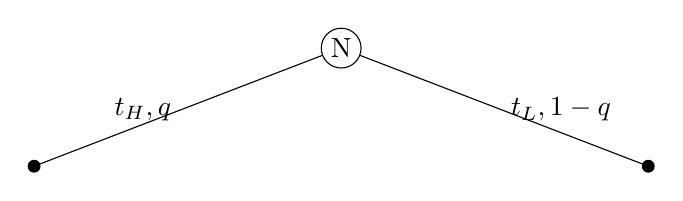
\begin{tikzpicture}[
				auto,
				level 1/.style={sibling distance=78mm},
				level 2/.style={sibling distance=10mm}]
			\tikzstyle{hollow node}=[circle,draw,inner sep=1.5]
			\tikzstyle{solid node}=[circle,draw,inner sep=1.5,fill=black]
			\node[hollow node]{N}
			child{node[solid node]{}
					edge from parent
					node[left]{$t_H, q$}
				}
			child{node[solid node]{}
					edge from parent
					node[right]{$t_L, 1-q$}
				}
			;
		\end{tikzpicture}
	\end{center}
	\vspace*{-1.4cm}
	\begin{center}
		\begin{minipage}[t]{0.48\linewidth}\centering
			\begin{game}[2][2]{Troncha}{Harry}
				& T & N \\
				T & $3000-y$,$y$ & 0, 2000\\
				N & 0, 2000      & 0, 2000\\
			\end{game}
		\end{minipage}\hfill%
		\begin{minipage}[t]{0.48\linewidth}\centering
			\begin{game}[2][2]{Troncha}{Harry}
				& T & N \\
				T & $1000-y$,$y$ & 0, 0\\
				N & 0, 0         & 0, 0\\
			\end{game}
		\end{minipage}
	\end{center}

	En donde la estrategia T es \textit{Trade} y N \textit{No Trade}. La utilidad esperada de Troncha si hay \textit{T} es

	\[
		\UE{Troncha}{T}=q(3000-y)+(1-q)(1000-y)
	\]

	Si no, la utilidad des de 0. Troncha estará dispuesta a comprar \textit{ssi} $\UE{Troncha}{T}\geq 0$

	\begin{align*}
		q(3000-y)+(1-q)(1000-y)            & \geq 0                                                                    \\
		3000q - qy + 1000 - y - 1000q + qy & \geq 0                                                                    \\
		2000q + 1000                       & \geq y, {\color{red}\text{ Notar q si } y < 2000 \text{ Harry no vende} } \\
		                                   & \therefore                                                                \\
		2000q + 1000                       & \geq y \geq 2000                                                          \\
		q \geq \frac{2000 - 1000}{2000}    & \geq \frac{1}{2}
	\end{align*}

	Es decir, a menos de que $q<1/2$, \textit{no existe} un equilibrio  en donde los coches buenos sean vendidos. Es decir, la proporción de coches malos debe ser menor del 50\%.

	Por ejemplo, suponiendo que $q=1/4$, ¿a qué precio estaría dispuesta a comprar Troncha? ¿Qué pasaría, a la larga, con un mercado así?

\end{exbox}

\subsection{Subasta al primer precio con pujadores aversos al riesgo}

En el ejemplo anterior de subasta en sobre cerrado al primer precio, modelamos dos jugadores neutrales al riesgo. Su puja fue de $b_i = ax_i$ con $a=1/2$. Ahora analizaremos un caso en donde la función de utilidad de los jugadores es cóncava, dada por

\begin{equation}
	u(w) = w^\alpha
	\label{eq:bern}
\end{equation}

La equación \ref{eq:bern} es una función de utilidad de Bernoulli, donde $0 < \alpha \leq 1$ es el parámetro de aversión al riesgo. De acuerdo con el coeficiente de aversión al riesgo de  Arrow-Pratt

\[
	r_A(w) = \frac{u''(w)}{u'(w)}
\]

$u'(w)=\alpha w^{\alpha - 1}$ y $u''(w)=\alpha (\alpha - 1) w^{\alpha - 2}$, con lo cual tendríamos un $r_A(w)$ de

\[
	r_A(w) = \frac{1-\alpha}{w}
\]

Cuando $\alpha = 1$, $r_A(w) = 0$, por lo que el jugador es neutral al riesgo.

\begin{exbox}{Subasta de sobre cerrado al primer precio (aversión al riesgo)}

	Encontrar la función óptima de puja $b_i(x_i)$ para $i=\{1, 2\}$, en donde los jugadores compiten por un objeto con su valuación $x_i \sim \text{uniforme}(0, 1)$. Explicar cómo esta función es afectada cuando $r_A(w)$ tiende a 1, con $\alpha \rightarrow 0$.

	\textbf{Sol.}

	Recordar que la fracción de $x_i$ que los jugadores pujan es $0 < a \leq 1$, y que el jugador $i$ gana solo si $b_i > b_j$, es decir, si $b_i > a x_j$, por lo que $p(\text{ganar}) = p(a x_j < b_i)$ o $p(x_j < b_i/a)$.

	Esta probabilidad es

	\[
		p(x_j < b_i/a) = \int_0^{b_i/a} dz = \Bigg[z\Bigg]_0^{b_i/a} = \frac{b_i}{a}
	\]

	\begin{center}
		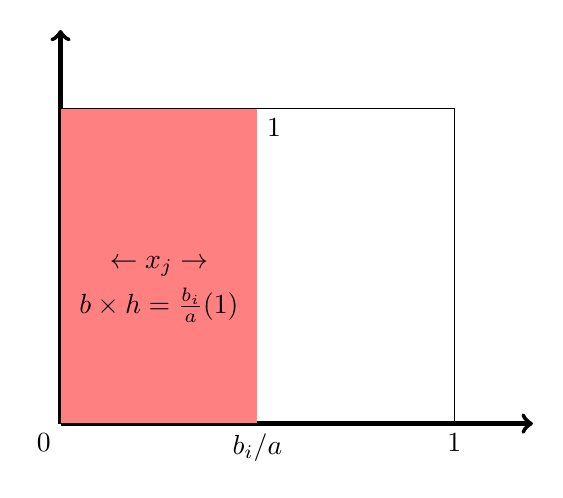
\begin{tikzpicture}
			\draw[->,ultra thick] (0,0)--(6,0);
			\draw[->,ultra thick] (0,0)--(0,5);
			\fill[red!50]    (0,0) rectangle  ++ (2.5,4) node[below right] {\color{black}$1$} ;
			\draw         (0,0) node[below left] {0} rectangle  ++ (5,4);
			\draw (5, 0) node[below] {$1$} (2.5, 0) node[below] {$b_i/a$};
			\draw (2.5/2,2) node {$\leftarrow x_j \rightarrow$};
			\draw (2.5/2,1.5) node {$b\times h = \frac{b_i}{a}(1)$};
		\end{tikzpicture}
	\end{center}

	Como vemos, la probabilidad no se ve afectada por la función de utilidad cóncava. Sabemos que la utilidad esperada del jugador $i$ está dada por

	\[
		\UE{i}{b_i}=p_i(\text{ganar})\times u_i(\text{ganar})
	\]

	Conocemos la primera. La utilidad de ganar está dada por $u_i(\text{ganar})=(x_i - b_i)^\alpha$. Por lo tanto

	\[
		\UE{i}{b_i}=\frac{b_i}{a}(x_i - b_i)^\alpha
	\]

	El jugador $i$ puja una cantidad $b_i^*$ que satisface

	\[
		b_i^* = \argmax_{0 < b_i \leq x_i}  \frac{b_i}{a}(x_i - b_i)^\alpha
	\]

	Tomando las CPO con respecto a $b_i$ tenemos%
	\footnote{
		Regla del producto: \[ [f(x)\cdot g(x)]'=f'(x)\cdot g'(x) \]
		Para nuestra función
		\[
			\frac{1}{a}\frac{\partial}{\partial b_i}b_i \Biggl(x_i - b_i)^\alpha\Biggr)
		\]

		Para el primero $f'(x) = \frac{\partial b_i}{\partial b_i} = 1$, y $g'(x)=\alpha(x_i-b_i)^{\alpha - 1}\frac{\partial(x_i-b_i)}{\partial b_i} = -\alpha(x_i-b_i)^{\alpha-1}$
	}

	\begin{align*}
		\frac{\partial}{\partial b_i} \Biggl( \frac{b_i}{a}(x_i - b_i)^\alpha\Biggr) & = 0                                                 \\
		\frac{1}{a}(x_i - b_i)^\alpha -\frac{b_i}{a}\alpha(x_i-b_x)^{\alpha - 1}     & =0                                                  \\
		\text{ simplificando }                                                       &                                                     \\
		b_i\alpha(x_i - b_i)^{\alpha - 1}                                            & = (x_i - b_i)^\alpha                                \\
		b_i\alpha                                                                    & = \frac{(x_i - b_i)^\alpha}{(x_i - b_i)^{\alpha-1}} \\
		b_i\alpha - b_i                                                              & = x_i                                               \\
		b_i^*                                                                        & = \frac{x_i}{1+\alpha}
	\end{align*}

	Notar que cuando $\alpha=1$, la puja óptima es $\frac{1}{2}x_i$. ¿Qué sucede si $\alpha$ disminuye?
	% funcion bid = x/(1 + alfa)
	\newcommand\bid[1]{x/(1 + #1)}
	% \begin{tikzpicture}
	%     \begin{axis}[grid=major, xmin=0, xmax=1, ymin=0, ymax=1, xlabel=$x_i$, ylabel=$b_i$];
	%     \foreach \a in {0.2, 0.4,..., 0.8}{
	%     \addplot [domain=0:1, samples=100, color=cyan]{(\bid{\a})};
	%     \expandafter\addlegendentry\expandafter{\a};
	%     };
	%     \end{axis}
	% \end{tikzpicture}

	\begin{center}
		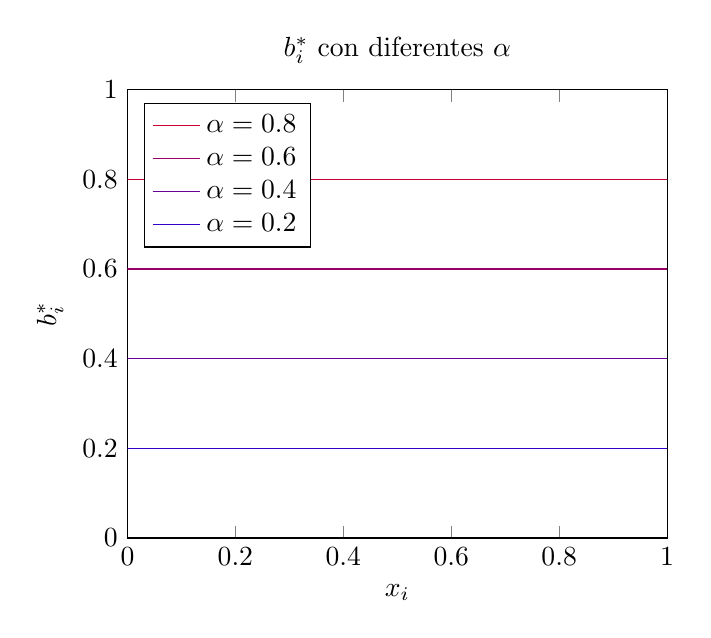
\begin{tikzpicture}
			\begin{axis}[%
					title={$b_i^*$ con diferentes $\alpha$},
					xmin=0,
					xmax=1,
					ymin=0,
					ymax=1,
					xlabel=$x_i$,
					ylabel=$b_i^*$,
					legend pos=north west
				]%
				\foreach [evaluate=\m as \redfrac using \m*100] \m in {0.8, 0.6, 0.4, 0.2}{
						\edef\temp{\noexpand\addplot[red!\redfrac!blue]{\bid{\m}};
							\noexpand\addlegendentry{$\alpha=\m$}}
						\temp
					}
			\end{axis}
		\end{tikzpicture}
	\end{center}

	\[
		\frac{\partial b_i^*}{\partial \alpha} =-\frac{x_i}{(1-\alpha)^2}
	\]

	Conforme $\alpha$ decrece, $b_i^*$ crece. Una función con $\alpha \rightarrow 1$ se aproxima más a una función identidad, de agentes neutrales al riesgo, con $a=1/2$. Notar que si $\alpha \rightarrow 1$, $b_i = x_i$. Los agentes aversos al riesgo tienen pujas más agresivas, para minimizar la probabilidad de perder la subasta.

	Considerar que el sujeto $j$ tiene un $\alpha = 0.9$, y un sujeto $i$ tiene un $\alpha=0.2$. La puja de $j$ será $\frac{1}{1.9}x_j$, mientras que la de $i$ será $\frac{1}{1.2}x_i$. La valuación del jugador $j$ debería ser al menos $\frac{1.9}{1.2}x_i$ para ganar (casi 1.6 veces el valor de $i$). Notar, sin embargo, que las utilidades de $i$ disminuyen conforme $\alpha \rightarrow 0$

	\newcommand\bidutil[1]{(x*(1-1/(1+#1)))^(#1)}

	\begin{center}
		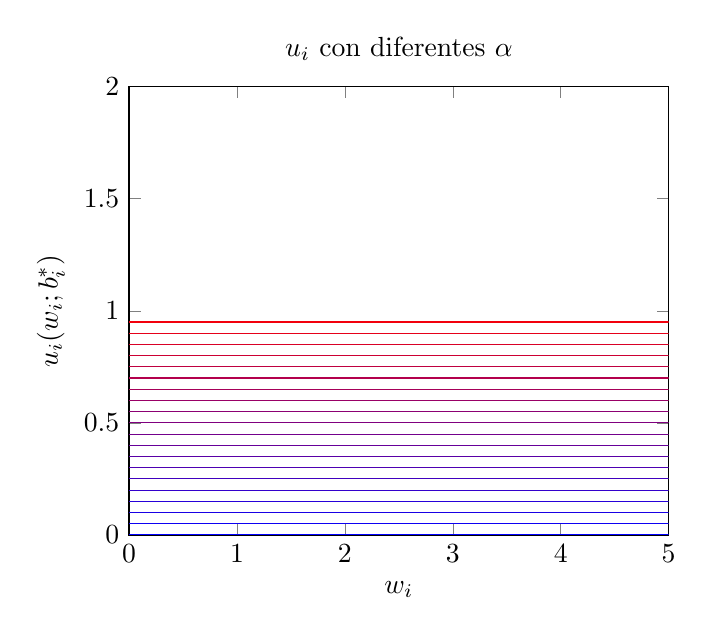
\begin{tikzpicture}
			\begin{axis}[%
					title={$u_i$ con diferentes $\alpha$},
					xmin=0,
					xmax=5,
					ymin=0,
					ymax=2,
					xlabel=$w_i$,
					ylabel=$u_i(w_i; b_i^*)$,
					legend pos=north west
				]%
				\foreach [evaluate=\m as \redfrac using \m*100] \m in {0,0.05, 0.1,...,1}{
						\edef\temp{\noexpand\addplot[red!\redfrac!blue]{\bidutil{\m}};}\temp
					}
			\end{axis}
		\end{tikzpicture}
	\end{center}

\end{exbox}

\begin{exbox}{Grupo de estudio}

	En un grupo de estudio con dos jugadores que se reunen a hacer su \sout{examen} tarea de teoría de juegos, cada uno puede esforzarse una cantidad $e_i=1$ o holgazanear $e_i=0$, con un costo de $c<1$ si se esfuerzan y de 0 si no. Si uno o ambos se esfuerzan, se obtiene éxito. Si no, fallan.

	Ambos varían respecto a su preocupación por el éxito educativo, que es su tipo $t_i \in [0, 1]$, que es $iid$ uniformemente en este intervalo, $t_i \sim \text{uniforme}(0,1)$. El valor del estudiante por éxito educativo está dado por el cuadrado de su tipo $t_i^2$. Si un estudiante escoge esforzarse, su utilidad sería $t_i^2 - c$. Si escoge holgazanear, su pago depende de lo que haga el compañero. Si el compañero $j$ se esfuerza, la ganancia de $i$ es $t_i^2$, mientras que si holgazanea, el pago es 0.

	Cada jugador necesita determinar si contribuir con esfuerzo basado en su tipo, en lo que cree sobre el tipo del otro jugador y en el costo de su esfuerzo.

	Podemos definir esta estrategia como $ s_i(ti) $ que mapea algún valor $t_i \in [0,1]$ a un esfuerzo correspondiente $ e_i \in \{0, 1\} $. De esta manera, $ s_i(t_i) $ retorna 0 (holgazanear) o 1 (contribuir), dependiendo del tipo $t_i$ escogido para el jugador $ i $.

	Sea $ p $ la probabilidad de que $ j $ contribuye con esfuerzo. Podemos definir la utilidad esperada del jugador $ i $ por holgazanear como

	$$ \underbrace{pt_i^2}_{j \text{ contribuye }} + \underbrace{(1-p)0}_{j \text{ holgazanea}} = pt_i^2 $$

	Si $ i $ contribuye, no importa qué haga $ j $, siempre obtendrá

	$$ t_i^2 - c $$

	Por lo tanto, la MR de $ i $ por esforzarse será esforzarse si su ganancia es \textit{al menos tan buena} como su ganancia esperada por holgazanear.

	$$ t_i^2 - c \geq pt_i^2 $$

	Resolviendo para $ t_i $,

	$$ t_i \geq \sqrt{\frac{c}{1-p}} $$

	La parte derecha es una constante. Esto implica que existe un umbral de $t_i$, $\hat{t}i$ por el cual el jugador $ i $ contribuye si $ t_i \geq \hat{t}_i $, pero no contribuye si $ t_i < \hat{t}_i $. Esto es una regla de umbral.

	Si el jugador $ i $ cree que $ j $ holgazaneará seguramente (i.e., $ p=0 $) responderá solamente si $ t_i \geq \sqrt{c} $, y dado que $ c<1 $ es posible que el jugador $ i $ contribuya si su compañero holgazanear.

	Por otro lado, si $ i $ cree que $ j $ se esforzará con probabilidad positiva (i.e., $ p > 0 $), podría hacer que $ \sqrt{\frac{c}{1-p}} $ sea mayor a 1. En ese caso, $ i $ nunca contribuirá dado que $ t_i \in [0, 1] $. El jugador preferirá un ``paseo gratis'' (parasitismo) y beneficiarse del esfuerzo de otros.

	Buscamos un ENB en el que cada estudiante tenga un umbral $ \hat{t}_i $ tal que

	\begin{align*}
		s_i(t_i)=\begin{cases}
			0 & \text{ si } t_i < \hat{t}_i \text{ (holgazanea)}    \\
			1 & \text{ si } t_i \geq \hat{t}_i \text{ (contribuye)}
		\end{cases}
	\end{align*}

	Ahora podemos derivar la MR del jugador $ i $ para algún valor de  $ \hat{t}_j $.
	Sabemos que $ j $ contribuye si $ t_j \geq \hat{t}_j $. ¿Cuál es esa probabilidad?

	$$ p(t_j \geq \hat{t}_j ) = 1 - p(t_j < \hat{t}_j) = 1-\hat{t}_j$$

	\begin{center}
		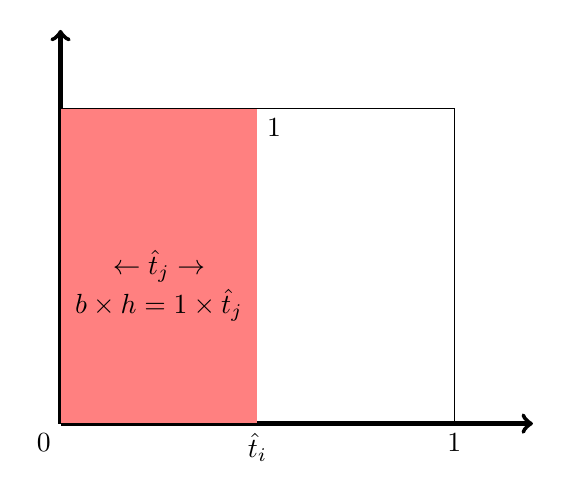
\begin{tikzpicture}
			\draw[->,ultra thick] (0,0)--(6,0);
			\draw[->,ultra thick] (0,0)--(0,5);
			\fill[red!50]    (0,0) rectangle  ++ (2.5,4) node[below right] {\color{black}$1$} ;
			\draw         (0,0) node[below left] {0} rectangle  ++ (5,4);
			\draw (5, 0) node[below] {$1$} (2.5, 0) node[below] {$\hat{t}_i$};
			\draw (2.5/2,2) node {$\leftarrow \hat{t}_j \rightarrow$};
			\draw (2.5/2,1.5) node {$b\times h = 1\times \hat{t}_j$};
		\end{tikzpicture}
	\end{center}

	Ahora, sabemos que $i$ contribuye si

	$$ t_i \geq \sqrt{\frac{c}{1-p}} = \sqrt{\frac{c}{1-(1-\hat{t}_j)}} = \sqrt{\frac{c}{\hat{t}_j}}$$

	\begin{myitemize}
		\item ¿Qué si $ \hat{t}_j > c $? Entonces, la parte derecha de la desigualdad será menor que 1, $ \sqrt{\frac{c}{\hat{t}j}} <1 $.
		\item ¿Qué si $ \hat{t}_j < c $? $ \sqrt{\frac{c}{\hat{t}j}} > 1 $
	\end{myitemize}

	%  \begin{center}
	%     % Created by tikzDevice version 0.12.3.1 on 2021-10-11 17:44:15
% !TEX encoding = UTF-8 Unicode
\begin{tikzpicture}[x=1pt,y=1pt]
\definecolor{fillColor}{RGB}{255,255,255}
\path[use as bounding box,fill=fillColor,fill opacity=0.00] (0,0) rectangle (216.81,216.81);
\begin{scope}
\path[clip] ( 27.60, 27.60) rectangle (204.81,204.81);
\definecolor{drawColor}{RGB}{223,83,107}

\path[draw=drawColor,line width= 0.8pt,line join=round,line cap=round] (1084.05, 29.10) --
	(1050.72, 29.19) --
	(998.22, 29.37) --
	(953.05, 29.55) --
	(913.65, 29.73) --
	(878.89, 29.90) --
	(847.92, 30.08) --
	(820.11, 30.26) --
	(794.94, 30.44) --
	(772.03, 30.61) --
	(751.06, 30.79) --
	(731.76, 30.97) --
	(713.93, 31.14) --
	(697.39, 31.32) --
	(681.99, 31.50) --
	(667.61, 31.68) --
	(654.13, 31.85) --
	(641.47, 32.03) --
	(629.55, 32.21) --
	(618.30, 32.38) --
	(607.66, 32.56) --
	(597.57, 32.74) --
	(587.99, 32.92) --
	(578.87, 33.09) --
	(570.19, 33.27) --
	(561.91, 33.45) --
	(553.99, 33.63) --
	(546.42, 33.80) --
	(539.16, 33.98) --
	(532.20, 34.16) --
	(525.52, 34.33) --
	(519.09, 34.51) --
	(512.91, 34.69) --
	(506.95, 34.87) --
	(501.21, 35.04) --
	(495.67, 35.22) --
	(490.32, 35.40) --
	(485.15, 35.57) --
	(480.15, 35.75) --
	(475.31, 35.93) --
	(470.63, 36.11) --
	(466.08, 36.28) --
	(461.67, 36.46) --
	(457.40, 36.64) --
	(453.24, 36.81) --
	(449.21, 36.99) --
	(445.29, 37.17) --
	(441.47, 37.35) --
	(437.76, 37.52) --
	(434.15, 37.70) --
	(430.63, 37.88) --
	(427.20, 38.06) --
	(423.85, 38.23) --
	(420.59, 38.41) --
	(417.41, 38.59) --
	(414.30, 38.76) --
	(411.27, 38.94) --
	(408.31, 39.12) --
	(405.41, 39.30) --
	(402.58, 39.47) --
	(399.82, 39.65) --
	(397.11, 39.83) --
	(394.46, 40.00) --
	(391.87, 40.18) --
	(389.33, 40.36) --
	(386.84, 40.54) --
	(384.41, 40.71) --
	(382.02, 40.89) --
	(379.68, 41.07) --
	(377.39, 41.25) --
	(375.14, 41.42) --
	(372.93, 41.60) --
	(370.77, 41.78) --
	(368.64, 41.95) --
	(366.55, 42.13) --
	(364.51, 42.31) --
	(362.50, 42.49) --
	(360.52, 42.66) --
	(358.58, 42.84) --
	(356.67, 43.02) --
	(354.80, 43.19) --
	(352.95, 43.37) --
	(351.14, 43.55) --
	(349.36, 43.73) --
	(347.60, 43.90) --
	(345.88, 44.08) --
	(344.18, 44.26) --
	(342.51, 44.43) --
	(340.87, 44.61) --
	(339.25, 44.79) --
	(337.65, 44.97) --
	(336.08, 45.14) --
	(334.54, 45.32) --
	(333.01, 45.50) --
	(331.51, 45.68) --
	(330.03, 45.85) --
	(328.58, 46.03) --
	(327.14, 46.21) --
	(325.72, 46.38) --
	(324.33, 46.56) --
	(322.95, 46.74) --
	(321.59, 46.92) --
	(320.25, 47.09) --
	(318.93, 47.27) --
	(317.63, 47.45) --
	(316.34, 47.62) --
	(315.07, 47.80) --
	(313.82, 47.98) --
	(312.58, 48.16) --
	(311.36, 48.33) --
	(310.16, 48.51) --
	(308.97, 48.69) --
	(307.79, 48.87) --
	(306.63, 49.04) --
	(305.49, 49.22) --
	(304.36, 49.40) --
	(303.24, 49.57) --
	(302.13, 49.75) --
	(301.04, 49.93) --
	(299.96, 50.11) --
	(298.90, 50.28) --
	(297.84, 50.46) --
	(296.80, 50.64) --
	(295.77, 50.81) --
	(294.75, 50.99) --
	(293.75, 51.17) --
	(292.75, 51.35) --
	(291.77, 51.52) --
	(290.80, 51.70) --
	(289.83, 51.88) --
	(288.88, 52.05) --
	(287.94, 52.23) --
	(287.01, 52.41) --
	(286.09, 52.59) --
	(285.18, 52.76) --
	(284.27, 52.94) --
	(283.38, 53.12) --
	(282.50, 53.30) --
	(281.62, 53.47) --
	(280.76, 53.65) --
	(279.90, 53.83) --
	(279.05, 54.00) --
	(278.21, 54.18) --
	(277.38, 54.36) --
	(276.56, 54.54) --
	(275.74, 54.71) --
	(274.94, 54.89) --
	(274.14, 55.07) --
	(273.35, 55.24) --
	(272.56, 55.42) --
	(271.79, 55.60) --
	(271.02, 55.78) --
	(270.25, 55.95) --
	(269.50, 56.13) --
	(268.75, 56.31) --
	(268.01, 56.49) --
	(267.28, 56.66) --
	(266.55, 56.84) --
	(265.83, 57.02) --
	(265.11, 57.19) --
	(264.41, 57.37) --
	(263.71, 57.55) --
	(263.01, 57.73) --
	(262.32, 57.90) --
	(261.64, 58.08) --
	(260.96, 58.26) --
	(260.29, 58.43) --
	(259.62, 58.61) --
	(258.96, 58.79) --
	(258.31, 58.97) --
	(257.66, 59.14) --
	(257.02, 59.32) --
	(256.38, 59.50) --
	(255.74, 59.68) --
	(255.12, 59.85) --
	(254.49, 60.03) --
	(253.88, 60.21) --
	(253.26, 60.38) --
	(252.66, 60.56) --
	(252.05, 60.74) --
	(251.46, 60.92) --
	(250.86, 61.09) --
	(250.28, 61.27) --
	(249.69, 61.45) --
	(249.11, 61.62) --
	(248.54, 61.80) --
	(247.97, 61.98) --
	(247.40, 62.16) --
	(246.84, 62.33) --
	(246.28, 62.51) --
	(245.73, 62.69) --
	(245.18, 62.86) --
	(244.64, 63.04) --
	(244.10, 63.22) --
	(243.56, 63.40) --
	(243.03, 63.57) --
	(242.50, 63.75) --
	(241.97, 63.93) --
	(241.45, 64.11) --
	(240.94, 64.28) --
	(240.42, 64.46) --
	(239.91, 64.64) --
	(239.41, 64.81) --
	(238.90, 64.99) --
	(238.41, 65.17) --
	(237.91, 65.35) --
	(237.42, 65.52) --
	(236.93, 65.70) --
	(236.44, 65.88) --
	(235.96, 66.05) --
	(235.48, 66.23) --
	(235.01, 66.41) --
	(234.54, 66.59) --
	(234.07, 66.76) --
	(233.60, 66.94) --
	(233.14, 67.12) --
	(232.68, 67.30) --
	(232.22, 67.47) --
	(231.77, 67.65) --
	(231.32, 67.83) --
	(230.87, 68.00) --
	(230.43, 68.18) --
	(229.99, 68.36) --
	(229.55, 68.54) --
	(229.11, 68.71) --
	(228.68, 68.89) --
	(228.25, 69.07) --
	(227.82, 69.24) --
	(227.40, 69.42) --
	(226.98, 69.60) --
	(226.56, 69.78) --
	(226.14, 69.95) --
	(225.73, 70.13) --
	(225.32, 70.31) --
	(224.91, 70.48) --
	(224.50, 70.66) --
	(224.10, 70.84) --
	(223.69, 71.02) --
	(223.30, 71.19) --
	(222.90, 71.37) --
	(222.51, 71.55) --
	(222.11, 71.73) --
	(221.72, 71.90) --
	(221.34, 72.08) --
	(220.95, 72.26) --
	(220.57, 72.43) --
	(220.19, 72.61) --
	(219.81, 72.79) --
	(219.44, 72.97) --
	(219.06, 73.14) --
	(218.69, 73.32) --
	(218.32, 73.50) --
	(217.95, 73.67) --
	(217.59, 73.85) --
	(217.23, 74.03) --
	(216.87, 74.21) --
	(216.51, 74.38) --
	(216.15, 74.56) --
	(215.79, 74.74) --
	(215.44, 74.92) --
	(215.09, 75.09) --
	(214.74, 75.27) --
	(214.40, 75.45) --
	(214.05, 75.62) --
	(213.71, 75.80) --
	(213.37, 75.98) --
	(213.03, 76.16) --
	(212.69, 76.33) --
	(212.35, 76.51) --
	(212.02, 76.69) --
	(211.69, 76.86) --
	(211.36, 77.04) --
	(211.03, 77.22) --
	(210.70, 77.40) --
	(210.38, 77.57) --
	(210.05, 77.75) --
	(209.73, 77.93) --
	(209.41, 78.10) --
	(209.10, 78.28) --
	(208.78, 78.46) --
	(208.46, 78.64) --
	(208.15, 78.81) --
	(207.84, 78.99) --
	(207.53, 79.17) --
	(207.22, 79.35) --
	(206.91, 79.52) --
	(206.61, 79.70) --
	(206.31, 79.88) --
	(206.00, 80.05) --
	(205.70, 80.23) --
	(205.40, 80.41) --
	(205.11, 80.59) --
	(204.81, 80.76) --
	(204.52, 80.94) --
	(204.22, 81.12) --
	(203.93, 81.29) --
	(203.64, 81.47) --
	(203.35, 81.65) --
	(203.06, 81.83) --
	(202.78, 82.00) --
	(202.49, 82.18) --
	(202.21, 82.36) --
	(201.93, 82.54) --
	(201.65, 82.71) --
	(201.37, 82.89) --
	(201.09, 83.07) --
	(200.81, 83.24) --
	(200.54, 83.42) --
	(200.27, 83.60) --
	(199.99, 83.78) --
	(199.72, 83.95) --
	(199.45, 84.13) --
	(199.18, 84.31) --
	(198.92, 84.48) --
	(198.65, 84.66) --
	(198.38, 84.84) --
	(198.12, 85.02) --
	(197.86, 85.19) --
	(197.60, 85.37) --
	(197.34, 85.55) --
	(197.08, 85.72) --
	(196.82, 85.90) --
	(196.56, 86.08) --
	(196.31, 86.26) --
	(196.05, 86.43) --
	(195.80, 86.61) --
	(195.55, 86.79) --
	(195.30, 86.97) --
	(195.05, 87.14) --
	(194.80, 87.32) --
	(194.55, 87.50) --
	(194.31, 87.67) --
	(194.06, 87.85) --
	(193.82, 88.03) --
	(193.57, 88.21) --
	(193.33, 88.38) --
	(193.09, 88.56) --
	(192.85, 88.74) --
	(192.61, 88.91) --
	(192.37, 89.09) --
	(192.14, 89.27) --
	(191.90, 89.45) --
	(191.66, 89.62) --
	(191.43, 89.80) --
	(191.20, 89.98) --
	(190.97, 90.16) --
	(190.74, 90.33) --
	(190.51, 90.51) --
	(190.28, 90.69) --
	(190.05, 90.86) --
	(189.82, 91.04) --
	(189.60, 91.22) --
	(189.37, 91.40) --
	(189.15, 91.57) --
	(188.92, 91.75) --
	(188.70, 91.93) --
	(188.48, 92.10) --
	(188.26, 92.28) --
	(188.04, 92.46) --
	(187.82, 92.64) --
	(187.60, 92.81) --
	(187.38, 92.99) --
	(187.17, 93.17) --
	(186.95, 93.34) --
	(186.74, 93.52) --
	(186.53, 93.70) --
	(186.31, 93.88) --
	(186.10, 94.05) --
	(185.89, 94.23) --
	(185.68, 94.41) --
	(185.47, 94.59) --
	(185.26, 94.76) --
	(185.06, 94.94) --
	(184.85, 95.12) --
	(184.64, 95.29) --
	(184.44, 95.47) --
	(184.23, 95.65) --
	(184.03, 95.83) --
	(183.83, 96.00) --
	(183.62, 96.18) --
	(183.42, 96.36) --
	(183.22, 96.53) --
	(183.02, 96.71) --
	(182.82, 96.89) --
	(182.63, 97.07) --
	(182.43, 97.24) --
	(182.23, 97.42) --
	(182.04, 97.60) --
	(181.84, 97.78) --
	(181.65, 97.95) --
	(181.45, 98.13) --
	(181.26, 98.31) --
	(181.07, 98.48) --
	(180.88, 98.66) --
	(180.69, 98.84) --
	(180.50, 99.02) --
	(180.31, 99.19) --
	(180.12, 99.37) --
	(179.93, 99.55) --
	(179.74, 99.72) --
	(179.56, 99.90) --
	(179.37,100.08) --
	(179.19,100.26) --
	(179.00,100.43) --
	(178.82,100.61) --
	(178.63,100.79) --
	(178.45,100.96) --
	(178.27,101.14) --
	(178.09,101.32) --
	(177.91,101.50) --
	(177.73,101.67) --
	(177.55,101.85) --
	(177.37,102.03) --
	(177.19,102.21) --
	(177.01,102.38) --
	(176.84,102.56) --
	(176.66,102.74) --
	(176.49,102.91) --
	(176.31,103.09) --
	(176.14,103.27) --
	(175.96,103.45) --
	(175.79,103.62) --
	(175.62,103.80) --
	(175.45,103.98) --
	(175.28,104.15) --
	(175.10,104.33) --
	(174.93,104.51) --
	(174.76,104.69) --
	(174.60,104.86) --
	(174.43,105.04) --
	(174.26,105.22) --
	(174.09,105.40) --
	(173.93,105.57) --
	(173.76,105.75) --
	(173.59,105.93) --
	(173.43,106.10) --
	(173.27,106.28) --
	(173.10,106.46) --
	(172.94,106.64) --
	(172.78,106.81) --
	(172.61,106.99) --
	(172.45,107.17) --
	(172.29,107.34) --
	(172.13,107.52) --
	(171.97,107.70) --
	(171.81,107.88) --
	(171.65,108.05) --
	(171.49,108.23) --
	(171.34,108.41) --
	(171.18,108.58) --
	(171.02,108.76) --
	(170.87,108.94) --
	(170.71,109.12) --
	(170.55,109.29) --
	(170.40,109.47) --
	(170.25,109.65) --
	(170.09,109.83) --
	(169.94,110.00) --
	(169.79,110.18) --
	(169.63,110.36) --
	(169.48,110.53) --
	(169.33,110.71) --
	(169.18,110.89) --
	(169.03,111.07) --
	(168.88,111.24) --
	(168.73,111.42) --
	(168.58,111.60) --
	(168.43,111.77) --
	(168.28,111.95) --
	(168.14,112.13) --
	(167.99,112.31) --
	(167.84,112.48) --
	(167.70,112.66) --
	(167.55,112.84) --
	(167.41,113.02) --
	(167.26,113.19) --
	(167.12,113.37) --
	(166.97,113.55) --
	(166.83,113.72) --
	(166.69,113.90) --
	(166.54,114.08) --
	(166.40,114.26) --
	(166.26,114.43) --
	(166.12,114.61) --
	(165.98,114.79) --
	(165.84,114.96) --
	(165.70,115.14) --
	(165.56,115.32) --
	(165.42,115.50) --
	(165.28,115.67) --
	(165.14,115.85) --
	(165.00,116.03) --
	(164.87,116.20) --
	(164.73,116.38) --
	(164.59,116.56) --
	(164.46,116.74) --
	(164.32,116.91) --
	(164.19,117.09) --
	(164.05,117.27) --
	(163.92,117.45) --
	(163.78,117.62) --
	(163.65,117.80) --
	(163.51,117.98) --
	(163.38,118.15) --
	(163.25,118.33) --
	(163.12,118.51) --
	(162.98,118.69) --
	(162.85,118.86) --
	(162.72,119.04) --
	(162.59,119.22) --
	(162.46,119.39) --
	(162.33,119.57) --
	(162.20,119.75) --
	(162.07,119.93) --
	(161.94,120.10) --
	(161.81,120.28) --
	(161.69,120.46) --
	(161.56,120.64) --
	(161.43,120.81) --
	(161.30,120.99) --
	(161.18,121.17) --
	(161.05,121.34) --
	(160.92,121.52) --
	(160.80,121.70) --
	(160.67,121.88) --
	(160.55,122.05) --
	(160.42,122.23) --
	(160.30,122.41) --
	(160.18,122.58) --
	(160.05,122.76) --
	(159.93,122.94) --
	(159.81,123.12) --
	(159.68,123.29) --
	(159.56,123.47) --
	(159.44,123.65) --
	(159.32,123.83) --
	(159.20,124.00) --
	(159.08,124.18) --
	(158.96,124.36) --
	(158.84,124.53) --
	(158.72,124.71) --
	(158.60,124.89) --
	(158.48,125.07) --
	(158.36,125.24) --
	(158.24,125.42) --
	(158.12,125.60) --
	(158.00,125.77) --
	(157.89,125.95) --
	(157.77,126.13) --
	(157.65,126.31) --
	(157.54,126.48) --
	(157.42,126.66) --
	(157.30,126.84) --
	(157.19,127.01) --
	(157.07,127.19) --
	(156.96,127.37) --
	(156.84,127.55) --
	(156.73,127.72) --
	(156.62,127.90) --
	(156.50,128.08) --
	(156.39,128.26) --
	(156.27,128.43) --
	(156.16,128.61) --
	(156.05,128.79) --
	(155.94,128.96) --
	(155.82,129.14) --
	(155.71,129.32) --
	(155.60,129.50) --
	(155.49,129.67) --
	(155.38,129.85) --
	(155.27,130.03) --
	(155.16,130.20) --
	(155.05,130.38) --
	(154.94,130.56) --
	(154.83,130.74) --
	(154.72,130.91) --
	(154.61,131.09) --
	(154.50,131.27) --
	(154.39,131.45) --
	(154.29,131.62) --
	(154.18,131.80) --
	(154.07,131.98) --
	(153.96,132.15) --
	(153.86,132.33) --
	(153.75,132.51) --
	(153.64,132.69) --
	(153.54,132.86) --
	(153.43,133.04) --
	(153.33,133.22) --
	(153.22,133.39) --
	(153.12,133.57) --
	(153.01,133.75) --
	(152.91,133.93) --
	(152.80,134.10) --
	(152.70,134.28) --
	(152.59,134.46) --
	(152.49,134.63) --
	(152.39,134.81) --
	(152.28,134.99) --
	(152.18,135.17) --
	(152.08,135.34) --
	(151.98,135.52) --
	(151.88,135.70) --
	(151.77,135.88) --
	(151.67,136.05) --
	(151.57,136.23) --
	(151.47,136.41) --
	(151.37,136.58) --
	(151.27,136.76) --
	(151.17,136.94) --
	(151.07,137.12) --
	(150.97,137.29) --
	(150.87,137.47) --
	(150.77,137.65) --
	(150.67,137.82) --
	(150.57,138.00) --
	(150.47,138.18) --
	(150.37,138.36) --
	(150.28,138.53) --
	(150.18,138.71) --
	(150.08,138.89) --
	(149.98,139.07) --
	(149.89,139.24) --
	(149.79,139.42) --
	(149.69,139.60) --
	(149.60,139.77) --
	(149.50,139.95) --
	(149.40,140.13) --
	(149.31,140.31) --
	(149.21,140.48) --
	(149.12,140.66) --
	(149.02,140.84) --
	(148.93,141.01) --
	(148.83,141.19) --
	(148.74,141.37) --
	(148.64,141.55) --
	(148.55,141.72) --
	(148.46,141.90) --
	(148.36,142.08) --
	(148.27,142.25) --
	(148.18,142.43) --
	(148.08,142.61) --
	(147.99,142.79) --
	(147.90,142.96) --
	(147.81,143.14) --
	(147.71,143.32) --
	(147.62,143.50) --
	(147.53,143.67) --
	(147.44,143.85) --
	(147.35,144.03) --
	(147.26,144.20) --
	(147.17,144.38) --
	(147.07,144.56) --
	(146.98,144.74) --
	(146.89,144.91) --
	(146.80,145.09) --
	(146.71,145.27) --
	(146.62,145.44) --
	(146.54,145.62) --
	(146.45,145.80) --
	(146.36,145.98) --
	(146.27,146.15) --
	(146.18,146.33) --
	(146.09,146.51) --
	(146.00,146.69) --
	(145.92,146.86) --
	(145.83,147.04) --
	(145.74,147.22) --
	(145.65,147.39) --
	(145.57,147.57) --
	(145.48,147.75) --
	(145.39,147.93) --
	(145.30,148.10) --
	(145.22,148.28) --
	(145.13,148.46) --
	(145.05,148.63) --
	(144.96,148.81) --
	(144.87,148.99) --
	(144.79,149.17) --
	(144.70,149.34) --
	(144.62,149.52) --
	(144.53,149.70) --
	(144.45,149.87) --
	(144.36,150.05) --
	(144.28,150.23) --
	(144.20,150.41) --
	(144.11,150.58) --
	(144.03,150.76) --
	(143.94,150.94) --
	(143.86,151.12) --
	(143.78,151.29) --
	(143.69,151.47) --
	(143.61,151.65) --
	(143.53,151.82) --
	(143.45,152.00) --
	(143.36,152.18) --
	(143.28,152.36) --
	(143.20,152.53) --
	(143.12,152.71) --
	(143.04,152.89) --
	(142.95,153.06) --
	(142.87,153.24) --
	(142.79,153.42) --
	(142.71,153.60) --
	(142.63,153.77) --
	(142.55,153.95) --
	(142.47,154.13) --
	(142.39,154.31) --
	(142.31,154.48) --
	(142.23,154.66) --
	(142.15,154.84) --
	(142.07,155.01) --
	(141.99,155.19) --
	(141.91,155.37) --
	(141.83,155.55) --
	(141.75,155.72) --
	(141.67,155.90) --
	(141.59,156.08) --
	(141.51,156.25) --
	(141.44,156.43) --
	(141.36,156.61) --
	(141.28,156.79) --
	(141.20,156.96) --
	(141.12,157.14) --
	(141.05,157.32) --
	(140.97,157.49) --
	(140.89,157.67) --
	(140.82,157.85) --
	(140.74,158.03) --
	(140.66,158.20) --
	(140.58,158.38) --
	(140.51,158.56) --
	(140.43,158.74) --
	(140.36,158.91) --
	(140.28,159.09) --
	(140.20,159.27) --
	(140.13,159.44) --
	(140.05,159.62) --
	(139.98,159.80) --
	(139.90,159.98) --
	(139.83,160.15) --
	(139.75,160.33) --
	(139.68,160.51) --
	(139.60,160.68) --
	(139.53,160.86) --
	(139.45,161.04) --
	(139.38,161.22) --
	(139.31,161.39) --
	(139.23,161.57) --
	(139.16,161.75) --
	(139.08,161.93) --
	(139.01,162.10) --
	(138.94,162.28) --
	(138.86,162.46) --
	(138.79,162.63) --
	(138.72,162.81) --
	(138.65,162.99) --
	(138.57,163.17) --
	(138.50,163.34) --
	(138.43,163.52) --
	(138.36,163.70) --
	(138.28,163.87) --
	(138.21,164.05) --
	(138.14,164.23) --
	(138.07,164.41) --
	(138.00,164.58) --
	(137.93,164.76) --
	(137.85,164.94) --
	(137.78,165.11) --
	(137.71,165.29) --
	(137.64,165.47) --
	(137.57,165.65) --
	(137.50,165.82) --
	(137.43,166.00) --
	(137.36,166.18) --
	(137.29,166.36) --
	(137.22,166.53) --
	(137.15,166.71) --
	(137.08,166.89) --
	(137.01,167.06) --
	(136.94,167.24) --
	(136.87,167.42) --
	(136.80,167.60) --
	(136.73,167.77) --
	(136.67,167.95) --
	(136.60,168.13) --
	(136.53,168.30) --
	(136.46,168.48) --
	(136.39,168.66) --
	(136.32,168.84) --
	(136.25,169.01) --
	(136.19,169.19) --
	(136.12,169.37) --
	(136.05,169.55) --
	(135.98,169.72) --
	(135.92,169.90) --
	(135.85,170.08) --
	(135.78,170.25) --
	(135.71,170.43) --
	(135.65,170.61) --
	(135.58,170.79) --
	(135.51,170.96) --
	(135.45,171.14) --
	(135.38,171.32) --
	(135.31,171.49) --
	(135.25,171.67) --
	(135.18,171.85) --
	(135.12,172.03) --
	(135.05,172.20) --
	(134.98,172.38) --
	(134.92,172.56) --
	(134.85,172.73) --
	(134.79,172.91) --
	(134.72,173.09) --
	(134.66,173.27) --
	(134.59,173.44) --
	(134.53,173.62) --
	(134.46,173.80) --
	(134.40,173.98) --
	(134.33,174.15) --
	(134.27,174.33) --
	(134.20,174.51) --
	(134.14,174.68) --
	(134.08,174.86) --
	(134.01,175.04) --
	(133.95,175.22) --
	(133.88,175.39) --
	(133.82,175.57) --
	(133.76,175.75) --
	(133.69,175.92) --
	(133.63,176.10) --
	(133.57,176.28) --
	(133.50,176.46) --
	(133.44,176.63) --
	(133.38,176.81) --
	(133.31,176.99) --
	(133.25,177.17) --
	(133.19,177.34) --
	(133.13,177.52) --
	(133.06,177.70) --
	(133.00,177.87) --
	(132.94,178.05) --
	(132.88,178.23) --
	(132.82,178.41) --
	(132.75,178.58) --
	(132.69,178.76) --
	(132.63,178.94) --
	(132.57,179.11) --
	(132.51,179.29) --
	(132.45,179.47) --
	(132.39,179.65) --
	(132.33,179.82) --
	(132.26,180.00) --
	(132.20,180.18) --
	(132.14,180.36) --
	(132.08,180.53) --
	(132.02,180.71) --
	(131.96,180.89) --
	(131.90,181.06) --
	(131.84,181.24) --
	(131.78,181.42) --
	(131.72,181.60) --
	(131.66,181.77) --
	(131.60,181.95) --
	(131.54,182.13) --
	(131.48,182.30) --
	(131.42,182.48) --
	(131.36,182.66) --
	(131.30,182.84) --
	(131.25,183.01) --
	(131.19,183.19) --
	(131.13,183.37) --
	(131.07,183.54) --
	(131.01,183.72) --
	(130.95,183.90) --
	(130.89,184.08) --
	(130.83,184.25) --
	(130.78,184.43) --
	(130.72,184.61) --
	(130.66,184.79) --
	(130.60,184.96) --
	(130.54,185.14) --
	(130.49,185.32) --
	(130.43,185.49) --
	(130.37,185.67) --
	(130.31,185.85) --
	(130.25,186.03) --
	(130.20,186.20) --
	(130.14,186.38) --
	(130.08,186.56) --
	(130.03,186.73) --
	(129.97,186.91) --
	(129.91,187.09) --
	(129.86,187.27) --
	(129.80,187.44) --
	(129.74,187.62) --
	(129.69,187.80) --
	(129.63,187.98) --
	(129.57,188.15) --
	(129.52,188.33) --
	(129.46,188.51) --
	(129.40,188.68) --
	(129.35,188.86) --
	(129.29,189.04) --
	(129.24,189.22) --
	(129.18,189.39) --
	(129.13,189.57) --
	(129.07,189.75) --
	(129.01,189.92) --
	(128.96,190.10) --
	(128.90,190.28) --
	(128.85,190.46) --
	(128.79,190.63) --
	(128.74,190.81) --
	(128.68,190.99) --
	(128.63,191.16) --
	(128.57,191.34) --
	(128.52,191.52) --
	(128.47,191.70) --
	(128.41,191.87) --
	(128.36,192.05) --
	(128.30,192.23) --
	(128.25,192.41) --
	(128.19,192.58) --
	(128.14,192.76) --
	(128.09,192.94) --
	(128.03,193.11) --
	(127.98,193.29) --
	(127.93,193.47) --
	(127.87,193.65) --
	(127.82,193.82) --
	(127.77,194.00) --
	(127.71,194.18) --
	(127.66,194.35) --
	(127.61,194.53) --
	(127.55,194.71) --
	(127.50,194.89) --
	(127.45,195.06) --
	(127.39,195.24) --
	(127.34,195.42) --
	(127.29,195.60) --
	(127.24,195.77) --
	(127.18,195.95) --
	(127.13,196.13) --
	(127.08,196.30) --
	(127.03,196.48) --
	(126.97,196.66) --
	(126.92,196.84) --
	(126.87,197.01) --
	(126.82,197.19) --
	(126.77,197.37) --
	(126.72,197.54) --
	(126.66,197.72) --
	(126.61,197.90) --
	(126.56,198.08) --
	(126.51,198.25) --
	(126.46,198.43) --
	(126.41,198.61) --
	(126.36,198.78) --
	(126.30,198.96) --
	(126.25,199.14) --
	(126.20,199.32) --
	(126.15,199.49) --
	(126.10,199.67) --
	(126.05,199.85) --
	(126.00,200.03) --
	(125.95,200.20) --
	(125.90,200.38) --
	(125.85,200.56) --
	(125.80,200.73) --
	(125.75,200.91) --
	(125.70,201.09) --
	(125.65,201.27) --
	(125.60,201.44) --
	(125.55,201.62) --
	(125.50,201.80) --
	(125.45,201.97) --
	(125.40,202.15) --
	(125.35,202.33) --
	(125.30,202.51) --
	(125.25,202.68) --
	(125.20,202.86) --
	(125.15,203.04) --
	(125.10,203.22) --
	(125.05,203.39) --
	(125.00,203.57) --
	(124.95,203.75) --
	(124.91,203.92) --
	(124.86,204.10) --
	(124.81,204.28) --
	(124.76,204.46) --
	(124.71,204.63) --
	(124.66,204.81);
\end{scope}
\begin{scope}
\path[clip] (  0.00,  0.00) rectangle (216.81,216.81);
\definecolor{drawColor}{RGB}{0,0,0}

\node[text=drawColor,anchor=base west,inner sep=0pt, outer sep=0pt, scale=  1.00] at (112.51,  7.51) {t};

\node[text=drawColor,anchor=base west,inner sep=0pt, outer sep=0pt, scale=  0.70] at (116.40,  6.00) {1};

\node[text=drawColor,rotate= 90.00,anchor=base west,inner sep=0pt, outer sep=0pt, scale=  1.00] at ( 11.69,112.51) {t};

\node[text=drawColor,rotate= 90.00,anchor=base west,inner sep=0pt, outer sep=0pt, scale=  0.70] at ( 13.20,116.40) {2};
\end{scope}
\begin{scope}
\path[clip] (  0.00,  0.00) rectangle (216.81,216.81);
\definecolor{drawColor}{RGB}{0,0,0}

\path[draw=drawColor,line width= 0.4pt,line join=round,line cap=round] ( 27.60, 27.60) -- (204.81, 27.60);

\path[draw=drawColor,line width= 0.4pt,line join=round,line cap=round] ( 27.60, 27.60) -- ( 27.60, 25.83);

\path[draw=drawColor,line width= 0.4pt,line join=round,line cap=round] (204.81, 27.60) -- (204.81, 25.83);

\node[text=drawColor,anchor=base,inner sep=0pt, outer sep=0pt, scale=  1.00] at ( 27.60, 12.00) {0};

\node[text=drawColor,anchor=base,inner sep=0pt, outer sep=0pt, scale=  1.00] at (204.81, 12.00) {1};

\path[draw=drawColor,line width= 0.4pt,line join=round,line cap=round] ( 27.60, 27.60) -- ( 27.60,204.81);

\path[draw=drawColor,line width= 0.4pt,line join=round,line cap=round] ( 27.60, 27.60) -- ( 25.83, 27.60);

\path[draw=drawColor,line width= 0.4pt,line join=round,line cap=round] ( 27.60,204.81) -- ( 25.83,204.81);

\node[text=drawColor,anchor=base east,inner sep=0pt, outer sep=0pt, scale=  1.00] at ( 21.60, 24.16) {0};

\node[text=drawColor,anchor=base east,inner sep=0pt, outer sep=0pt, scale=  1.00] at ( 21.60,201.37) {1};

\path[draw=drawColor,line width= 0.4pt,line join=round,line cap=round] ( 27.60, 27.60) --
	(204.81, 27.60) --
	(204.81,204.81) --
	( 27.60,204.81) --
	cycle;
\end{scope}
\begin{scope}
\path[clip] ( 27.60, 27.60) rectangle (204.81,204.81);
\definecolor{drawColor}{RGB}{0,0,0}

\path[draw=drawColor,line width= 0.4pt,dash pattern=on 4pt off 4pt ,line join=round,line cap=round] ( 27.60,124.66) -- (204.81,124.66);

\path[draw=drawColor,line width= 0.4pt,dash pattern=on 4pt off 4pt ,line join=round,line cap=round] ( 80.76, 27.60) -- ( 80.76,204.81);
\definecolor{drawColor}{RGB}{34,151,230}

\path[draw=drawColor,line width= 0.8pt,line join=round,line cap=round] ( 29.10,1084.05) --
	( 29.19,1050.72) --
	( 29.37,998.22) --
	( 29.55,953.05) --
	( 29.73,913.65) --
	( 29.90,878.89) --
	( 30.08,847.92) --
	( 30.26,820.11) --
	( 30.44,794.94) --
	( 30.61,772.03) --
	( 30.79,751.06) --
	( 30.97,731.76) --
	( 31.14,713.93) --
	( 31.32,697.39) --
	( 31.50,681.99) --
	( 31.68,667.61) --
	( 31.85,654.13) --
	( 32.03,641.47) --
	( 32.21,629.55) --
	( 32.38,618.30) --
	( 32.56,607.66) --
	( 32.74,597.57) --
	( 32.92,587.99) --
	( 33.09,578.87) --
	( 33.27,570.19) --
	( 33.45,561.91) --
	( 33.63,553.99) --
	( 33.80,546.42) --
	( 33.98,539.16) --
	( 34.16,532.20) --
	( 34.33,525.52) --
	( 34.51,519.09) --
	( 34.69,512.91) --
	( 34.87,506.95) --
	( 35.04,501.21) --
	( 35.22,495.67) --
	( 35.40,490.32) --
	( 35.57,485.15) --
	( 35.75,480.15) --
	( 35.93,475.31) --
	( 36.11,470.63) --
	( 36.28,466.08) --
	( 36.46,461.67) --
	( 36.64,457.40) --
	( 36.81,453.24) --
	( 36.99,449.21) --
	( 37.17,445.29) --
	( 37.35,441.47) --
	( 37.52,437.76) --
	( 37.70,434.15) --
	( 37.88,430.63) --
	( 38.06,427.20) --
	( 38.23,423.85) --
	( 38.41,420.59) --
	( 38.59,417.41) --
	( 38.76,414.30) --
	( 38.94,411.27) --
	( 39.12,408.31) --
	( 39.30,405.41) --
	( 39.47,402.58) --
	( 39.65,399.82) --
	( 39.83,397.11) --
	( 40.00,394.46) --
	( 40.18,391.87) --
	( 40.36,389.33) --
	( 40.54,386.84) --
	( 40.71,384.41) --
	( 40.89,382.02) --
	( 41.07,379.68) --
	( 41.25,377.39) --
	( 41.42,375.14) --
	( 41.60,372.93) --
	( 41.78,370.77) --
	( 41.95,368.64) --
	( 42.13,366.55) --
	( 42.31,364.51) --
	( 42.49,362.50) --
	( 42.66,360.52) --
	( 42.84,358.58) --
	( 43.02,356.67) --
	( 43.19,354.80) --
	( 43.37,352.95) --
	( 43.55,351.14) --
	( 43.73,349.36) --
	( 43.90,347.60) --
	( 44.08,345.88) --
	( 44.26,344.18) --
	( 44.43,342.51) --
	( 44.61,340.87) --
	( 44.79,339.25) --
	( 44.97,337.65) --
	( 45.14,336.08) --
	( 45.32,334.54) --
	( 45.50,333.01) --
	( 45.68,331.51) --
	( 45.85,330.03) --
	( 46.03,328.58) --
	( 46.21,327.14) --
	( 46.38,325.72) --
	( 46.56,324.33) --
	( 46.74,322.95) --
	( 46.92,321.59) --
	( 47.09,320.25) --
	( 47.27,318.93) --
	( 47.45,317.63) --
	( 47.62,316.34) --
	( 47.80,315.07) --
	( 47.98,313.82) --
	( 48.16,312.58) --
	( 48.33,311.36) --
	( 48.51,310.16) --
	( 48.69,308.97) --
	( 48.87,307.79) --
	( 49.04,306.63) --
	( 49.22,305.49) --
	( 49.40,304.36) --
	( 49.57,303.24) --
	( 49.75,302.13) --
	( 49.93,301.04) --
	( 50.11,299.96) --
	( 50.28,298.90) --
	( 50.46,297.84) --
	( 50.64,296.80) --
	( 50.81,295.77) --
	( 50.99,294.75) --
	( 51.17,293.75) --
	( 51.35,292.75) --
	( 51.52,291.77) --
	( 51.70,290.80) --
	( 51.88,289.83) --
	( 52.05,288.88) --
	( 52.23,287.94) --
	( 52.41,287.01) --
	( 52.59,286.09) --
	( 52.76,285.18) --
	( 52.94,284.27) --
	( 53.12,283.38) --
	( 53.30,282.50) --
	( 53.47,281.62) --
	( 53.65,280.76) --
	( 53.83,279.90) --
	( 54.00,279.05) --
	( 54.18,278.21) --
	( 54.36,277.38) --
	( 54.54,276.56) --
	( 54.71,275.74) --
	( 54.89,274.94) --
	( 55.07,274.14) --
	( 55.24,273.35) --
	( 55.42,272.56) --
	( 55.60,271.79) --
	( 55.78,271.02) --
	( 55.95,270.25) --
	( 56.13,269.50) --
	( 56.31,268.75) --
	( 56.49,268.01) --
	( 56.66,267.28) --
	( 56.84,266.55) --
	( 57.02,265.83) --
	( 57.19,265.11) --
	( 57.37,264.41) --
	( 57.55,263.71) --
	( 57.73,263.01) --
	( 57.90,262.32) --
	( 58.08,261.64) --
	( 58.26,260.96) --
	( 58.43,260.29) --
	( 58.61,259.62) --
	( 58.79,258.96) --
	( 58.97,258.31) --
	( 59.14,257.66) --
	( 59.32,257.02) --
	( 59.50,256.38) --
	( 59.68,255.74) --
	( 59.85,255.12) --
	( 60.03,254.49) --
	( 60.21,253.88) --
	( 60.38,253.26) --
	( 60.56,252.66) --
	( 60.74,252.05) --
	( 60.92,251.46) --
	( 61.09,250.86) --
	( 61.27,250.28) --
	( 61.45,249.69) --
	( 61.62,249.11) --
	( 61.80,248.54) --
	( 61.98,247.97) --
	( 62.16,247.40) --
	( 62.33,246.84) --
	( 62.51,246.28) --
	( 62.69,245.73) --
	( 62.86,245.18) --
	( 63.04,244.64) --
	( 63.22,244.10) --
	( 63.40,243.56) --
	( 63.57,243.03) --
	( 63.75,242.50) --
	( 63.93,241.97) --
	( 64.11,241.45) --
	( 64.28,240.94) --
	( 64.46,240.42) --
	( 64.64,239.91) --
	( 64.81,239.41) --
	( 64.99,238.90) --
	( 65.17,238.41) --
	( 65.35,237.91) --
	( 65.52,237.42) --
	( 65.70,236.93) --
	( 65.88,236.44) --
	( 66.05,235.96) --
	( 66.23,235.48) --
	( 66.41,235.01) --
	( 66.59,234.54) --
	( 66.76,234.07) --
	( 66.94,233.60) --
	( 67.12,233.14) --
	( 67.30,232.68) --
	( 67.47,232.22) --
	( 67.65,231.77) --
	( 67.83,231.32) --
	( 68.00,230.87) --
	( 68.18,230.43) --
	( 68.36,229.99) --
	( 68.54,229.55) --
	( 68.71,229.11) --
	( 68.89,228.68) --
	( 69.07,228.25) --
	( 69.24,227.82) --
	( 69.42,227.40) --
	( 69.60,226.98) --
	( 69.78,226.56) --
	( 69.95,226.14) --
	( 70.13,225.73) --
	( 70.31,225.32) --
	( 70.48,224.91) --
	( 70.66,224.50) --
	( 70.84,224.10) --
	( 71.02,223.69) --
	( 71.19,223.30) --
	( 71.37,222.90) --
	( 71.55,222.51) --
	( 71.73,222.11) --
	( 71.90,221.72) --
	( 72.08,221.34) --
	( 72.26,220.95) --
	( 72.43,220.57) --
	( 72.61,220.19) --
	( 72.79,219.81) --
	( 72.97,219.44) --
	( 73.14,219.06) --
	( 73.32,218.69) --
	( 73.50,218.32) --
	( 73.67,217.95) --
	( 73.85,217.59) --
	( 74.03,217.23) --
	( 74.21,216.87) --
	( 74.38,216.51) --
	( 74.56,216.15) --
	( 74.74,215.79) --
	( 74.92,215.44) --
	( 75.09,215.09) --
	( 75.27,214.74) --
	( 75.45,214.40) --
	( 75.62,214.05) --
	( 75.80,213.71) --
	( 75.98,213.37) --
	( 76.16,213.03) --
	( 76.33,212.69) --
	( 76.51,212.35) --
	( 76.69,212.02) --
	( 76.86,211.69) --
	( 77.04,211.36) --
	( 77.22,211.03) --
	( 77.40,210.70) --
	( 77.57,210.38) --
	( 77.75,210.05) --
	( 77.93,209.73) --
	( 78.10,209.41) --
	( 78.28,209.10) --
	( 78.46,208.78) --
	( 78.64,208.46) --
	( 78.81,208.15) --
	( 78.99,207.84) --
	( 79.17,207.53) --
	( 79.35,207.22) --
	( 79.52,206.91) --
	( 79.70,206.61) --
	( 79.88,206.31) --
	( 80.05,206.00) --
	( 80.23,205.70) --
	( 80.41,205.40) --
	( 80.59,205.11) --
	( 80.76,204.81) --
	( 80.94,204.52) --
	( 81.12,204.22) --
	( 81.29,203.93) --
	( 81.47,203.64) --
	( 81.65,203.35) --
	( 81.83,203.06) --
	( 82.00,202.78) --
	( 82.18,202.49) --
	( 82.36,202.21) --
	( 82.54,201.93) --
	( 82.71,201.65) --
	( 82.89,201.37) --
	( 83.07,201.09) --
	( 83.24,200.81) --
	( 83.42,200.54) --
	( 83.60,200.27) --
	( 83.78,199.99) --
	( 83.95,199.72) --
	( 84.13,199.45) --
	( 84.31,199.18) --
	( 84.48,198.92) --
	( 84.66,198.65) --
	( 84.84,198.38) --
	( 85.02,198.12) --
	( 85.19,197.86) --
	( 85.37,197.60) --
	( 85.55,197.34) --
	( 85.72,197.08) --
	( 85.90,196.82) --
	( 86.08,196.56) --
	( 86.26,196.31) --
	( 86.43,196.05) --
	( 86.61,195.80) --
	( 86.79,195.55) --
	( 86.97,195.30) --
	( 87.14,195.05) --
	( 87.32,194.80) --
	( 87.50,194.55) --
	( 87.67,194.31) --
	( 87.85,194.06) --
	( 88.03,193.82) --
	( 88.21,193.57) --
	( 88.38,193.33) --
	( 88.56,193.09) --
	( 88.74,192.85) --
	( 88.91,192.61) --
	( 89.09,192.37) --
	( 89.27,192.14) --
	( 89.45,191.90) --
	( 89.62,191.66) --
	( 89.80,191.43) --
	( 89.98,191.20) --
	( 90.16,190.97) --
	( 90.33,190.74) --
	( 90.51,190.51) --
	( 90.69,190.28) --
	( 90.86,190.05) --
	( 91.04,189.82) --
	( 91.22,189.60) --
	( 91.40,189.37) --
	( 91.57,189.15) --
	( 91.75,188.92) --
	( 91.93,188.70) --
	( 92.10,188.48) --
	( 92.28,188.26) --
	( 92.46,188.04) --
	( 92.64,187.82) --
	( 92.81,187.60) --
	( 92.99,187.38) --
	( 93.17,187.17) --
	( 93.34,186.95) --
	( 93.52,186.74) --
	( 93.70,186.53) --
	( 93.88,186.31) --
	( 94.05,186.10) --
	( 94.23,185.89) --
	( 94.41,185.68) --
	( 94.59,185.47) --
	( 94.76,185.26) --
	( 94.94,185.06) --
	( 95.12,184.85) --
	( 95.29,184.64) --
	( 95.47,184.44) --
	( 95.65,184.23) --
	( 95.83,184.03) --
	( 96.00,183.83) --
	( 96.18,183.62) --
	( 96.36,183.42) --
	( 96.53,183.22) --
	( 96.71,183.02) --
	( 96.89,182.82) --
	( 97.07,182.63) --
	( 97.24,182.43) --
	( 97.42,182.23) --
	( 97.60,182.04) --
	( 97.78,181.84) --
	( 97.95,181.65) --
	( 98.13,181.45) --
	( 98.31,181.26) --
	( 98.48,181.07) --
	( 98.66,180.88) --
	( 98.84,180.69) --
	( 99.02,180.50) --
	( 99.19,180.31) --
	( 99.37,180.12) --
	( 99.55,179.93) --
	( 99.72,179.74) --
	( 99.90,179.56) --
	(100.08,179.37) --
	(100.26,179.19) --
	(100.43,179.00) --
	(100.61,178.82) --
	(100.79,178.63) --
	(100.96,178.45) --
	(101.14,178.27) --
	(101.32,178.09) --
	(101.50,177.91) --
	(101.67,177.73) --
	(101.85,177.55) --
	(102.03,177.37) --
	(102.21,177.19) --
	(102.38,177.01) --
	(102.56,176.84) --
	(102.74,176.66) --
	(102.91,176.49) --
	(103.09,176.31) --
	(103.27,176.14) --
	(103.45,175.96) --
	(103.62,175.79) --
	(103.80,175.62) --
	(103.98,175.45) --
	(104.15,175.28) --
	(104.33,175.10) --
	(104.51,174.93) --
	(104.69,174.76) --
	(104.86,174.60) --
	(105.04,174.43) --
	(105.22,174.26) --
	(105.40,174.09) --
	(105.57,173.93) --
	(105.75,173.76) --
	(105.93,173.59) --
	(106.10,173.43) --
	(106.28,173.27) --
	(106.46,173.10) --
	(106.64,172.94) --
	(106.81,172.78) --
	(106.99,172.61) --
	(107.17,172.45) --
	(107.34,172.29) --
	(107.52,172.13) --
	(107.70,171.97) --
	(107.88,171.81) --
	(108.05,171.65) --
	(108.23,171.49) --
	(108.41,171.34) --
	(108.58,171.18) --
	(108.76,171.02) --
	(108.94,170.87) --
	(109.12,170.71) --
	(109.29,170.55) --
	(109.47,170.40) --
	(109.65,170.25) --
	(109.83,170.09) --
	(110.00,169.94) --
	(110.18,169.79) --
	(110.36,169.63) --
	(110.53,169.48) --
	(110.71,169.33) --
	(110.89,169.18) --
	(111.07,169.03) --
	(111.24,168.88) --
	(111.42,168.73) --
	(111.60,168.58) --
	(111.77,168.43) --
	(111.95,168.28) --
	(112.13,168.14) --
	(112.31,167.99) --
	(112.48,167.84) --
	(112.66,167.70) --
	(112.84,167.55) --
	(113.02,167.41) --
	(113.19,167.26) --
	(113.37,167.12) --
	(113.55,166.97) --
	(113.72,166.83) --
	(113.90,166.69) --
	(114.08,166.54) --
	(114.26,166.40) --
	(114.43,166.26) --
	(114.61,166.12) --
	(114.79,165.98) --
	(114.96,165.84) --
	(115.14,165.70) --
	(115.32,165.56) --
	(115.50,165.42) --
	(115.67,165.28) --
	(115.85,165.14) --
	(116.03,165.00) --
	(116.20,164.87) --
	(116.38,164.73) --
	(116.56,164.59) --
	(116.74,164.46) --
	(116.91,164.32) --
	(117.09,164.19) --
	(117.27,164.05) --
	(117.45,163.92) --
	(117.62,163.78) --
	(117.80,163.65) --
	(117.98,163.51) --
	(118.15,163.38) --
	(118.33,163.25) --
	(118.51,163.12) --
	(118.69,162.98) --
	(118.86,162.85) --
	(119.04,162.72) --
	(119.22,162.59) --
	(119.39,162.46) --
	(119.57,162.33) --
	(119.75,162.20) --
	(119.93,162.07) --
	(120.10,161.94) --
	(120.28,161.81) --
	(120.46,161.69) --
	(120.64,161.56) --
	(120.81,161.43) --
	(120.99,161.30) --
	(121.17,161.18) --
	(121.34,161.05) --
	(121.52,160.92) --
	(121.70,160.80) --
	(121.88,160.67) --
	(122.05,160.55) --
	(122.23,160.42) --
	(122.41,160.30) --
	(122.58,160.18) --
	(122.76,160.05) --
	(122.94,159.93) --
	(123.12,159.81) --
	(123.29,159.68) --
	(123.47,159.56) --
	(123.65,159.44) --
	(123.83,159.32) --
	(124.00,159.20) --
	(124.18,159.08) --
	(124.36,158.96) --
	(124.53,158.84) --
	(124.71,158.72) --
	(124.89,158.60) --
	(125.07,158.48) --
	(125.24,158.36) --
	(125.42,158.24) --
	(125.60,158.12) --
	(125.77,158.00) --
	(125.95,157.89) --
	(126.13,157.77) --
	(126.31,157.65) --
	(126.48,157.54) --
	(126.66,157.42) --
	(126.84,157.30) --
	(127.01,157.19) --
	(127.19,157.07) --
	(127.37,156.96) --
	(127.55,156.84) --
	(127.72,156.73) --
	(127.90,156.62) --
	(128.08,156.50) --
	(128.26,156.39) --
	(128.43,156.27) --
	(128.61,156.16) --
	(128.79,156.05) --
	(128.96,155.94) --
	(129.14,155.82) --
	(129.32,155.71) --
	(129.50,155.60) --
	(129.67,155.49) --
	(129.85,155.38) --
	(130.03,155.27) --
	(130.20,155.16) --
	(130.38,155.05) --
	(130.56,154.94) --
	(130.74,154.83) --
	(130.91,154.72) --
	(131.09,154.61) --
	(131.27,154.50) --
	(131.45,154.39) --
	(131.62,154.29) --
	(131.80,154.18) --
	(131.98,154.07) --
	(132.15,153.96) --
	(132.33,153.86) --
	(132.51,153.75) --
	(132.69,153.64) --
	(132.86,153.54) --
	(133.04,153.43) --
	(133.22,153.33) --
	(133.39,153.22) --
	(133.57,153.12) --
	(133.75,153.01) --
	(133.93,152.91) --
	(134.10,152.80) --
	(134.28,152.70) --
	(134.46,152.59) --
	(134.63,152.49) --
	(134.81,152.39) --
	(134.99,152.28) --
	(135.17,152.18) --
	(135.34,152.08) --
	(135.52,151.98) --
	(135.70,151.88) --
	(135.88,151.77) --
	(136.05,151.67) --
	(136.23,151.57) --
	(136.41,151.47) --
	(136.58,151.37) --
	(136.76,151.27) --
	(136.94,151.17) --
	(137.12,151.07) --
	(137.29,150.97) --
	(137.47,150.87) --
	(137.65,150.77) --
	(137.82,150.67) --
	(138.00,150.57) --
	(138.18,150.47) --
	(138.36,150.37) --
	(138.53,150.28) --
	(138.71,150.18) --
	(138.89,150.08) --
	(139.07,149.98) --
	(139.24,149.89) --
	(139.42,149.79) --
	(139.60,149.69) --
	(139.77,149.60) --
	(139.95,149.50) --
	(140.13,149.40) --
	(140.31,149.31) --
	(140.48,149.21) --
	(140.66,149.12) --
	(140.84,149.02) --
	(141.01,148.93) --
	(141.19,148.83) --
	(141.37,148.74) --
	(141.55,148.64) --
	(141.72,148.55) --
	(141.90,148.46) --
	(142.08,148.36) --
	(142.25,148.27) --
	(142.43,148.18) --
	(142.61,148.08) --
	(142.79,147.99) --
	(142.96,147.90) --
	(143.14,147.81) --
	(143.32,147.71) --
	(143.50,147.62) --
	(143.67,147.53) --
	(143.85,147.44) --
	(144.03,147.35) --
	(144.20,147.26) --
	(144.38,147.17) --
	(144.56,147.07) --
	(144.74,146.98) --
	(144.91,146.89) --
	(145.09,146.80) --
	(145.27,146.71) --
	(145.44,146.62) --
	(145.62,146.54) --
	(145.80,146.45) --
	(145.98,146.36) --
	(146.15,146.27) --
	(146.33,146.18) --
	(146.51,146.09) --
	(146.69,146.00) --
	(146.86,145.92) --
	(147.04,145.83) --
	(147.22,145.74) --
	(147.39,145.65) --
	(147.57,145.57) --
	(147.75,145.48) --
	(147.93,145.39) --
	(148.10,145.30) --
	(148.28,145.22) --
	(148.46,145.13) --
	(148.63,145.05) --
	(148.81,144.96) --
	(148.99,144.87) --
	(149.17,144.79) --
	(149.34,144.70) --
	(149.52,144.62) --
	(149.70,144.53) --
	(149.87,144.45) --
	(150.05,144.36) --
	(150.23,144.28) --
	(150.41,144.20) --
	(150.58,144.11) --
	(150.76,144.03) --
	(150.94,143.94) --
	(151.12,143.86) --
	(151.29,143.78) --
	(151.47,143.69) --
	(151.65,143.61) --
	(151.82,143.53) --
	(152.00,143.45) --
	(152.18,143.36) --
	(152.36,143.28) --
	(152.53,143.20) --
	(152.71,143.12) --
	(152.89,143.04) --
	(153.06,142.95) --
	(153.24,142.87) --
	(153.42,142.79) --
	(153.60,142.71) --
	(153.77,142.63) --
	(153.95,142.55) --
	(154.13,142.47) --
	(154.31,142.39) --
	(154.48,142.31) --
	(154.66,142.23) --
	(154.84,142.15) --
	(155.01,142.07) --
	(155.19,141.99) --
	(155.37,141.91) --
	(155.55,141.83) --
	(155.72,141.75) --
	(155.90,141.67) --
	(156.08,141.59) --
	(156.25,141.51) --
	(156.43,141.44) --
	(156.61,141.36) --
	(156.79,141.28) --
	(156.96,141.20) --
	(157.14,141.12) --
	(157.32,141.05) --
	(157.49,140.97) --
	(157.67,140.89) --
	(157.85,140.82) --
	(158.03,140.74) --
	(158.20,140.66) --
	(158.38,140.58) --
	(158.56,140.51) --
	(158.74,140.43) --
	(158.91,140.36) --
	(159.09,140.28) --
	(159.27,140.20) --
	(159.44,140.13) --
	(159.62,140.05) --
	(159.80,139.98) --
	(159.98,139.90) --
	(160.15,139.83) --
	(160.33,139.75) --
	(160.51,139.68) --
	(160.68,139.60) --
	(160.86,139.53) --
	(161.04,139.45) --
	(161.22,139.38) --
	(161.39,139.31) --
	(161.57,139.23) --
	(161.75,139.16) --
	(161.93,139.08) --
	(162.10,139.01) --
	(162.28,138.94) --
	(162.46,138.86) --
	(162.63,138.79) --
	(162.81,138.72) --
	(162.99,138.65) --
	(163.17,138.57) --
	(163.34,138.50) --
	(163.52,138.43) --
	(163.70,138.36) --
	(163.87,138.28) --
	(164.05,138.21) --
	(164.23,138.14) --
	(164.41,138.07) --
	(164.58,138.00) --
	(164.76,137.93) --
	(164.94,137.85) --
	(165.11,137.78) --
	(165.29,137.71) --
	(165.47,137.64) --
	(165.65,137.57) --
	(165.82,137.50) --
	(166.00,137.43) --
	(166.18,137.36) --
	(166.36,137.29) --
	(166.53,137.22) --
	(166.71,137.15) --
	(166.89,137.08) --
	(167.06,137.01) --
	(167.24,136.94) --
	(167.42,136.87) --
	(167.60,136.80) --
	(167.77,136.73) --
	(167.95,136.67) --
	(168.13,136.60) --
	(168.30,136.53) --
	(168.48,136.46) --
	(168.66,136.39) --
	(168.84,136.32) --
	(169.01,136.25) --
	(169.19,136.19) --
	(169.37,136.12) --
	(169.55,136.05) --
	(169.72,135.98) --
	(169.90,135.92) --
	(170.08,135.85) --
	(170.25,135.78) --
	(170.43,135.71) --
	(170.61,135.65) --
	(170.79,135.58) --
	(170.96,135.51) --
	(171.14,135.45) --
	(171.32,135.38) --
	(171.49,135.31) --
	(171.67,135.25) --
	(171.85,135.18) --
	(172.03,135.12) --
	(172.20,135.05) --
	(172.38,134.98) --
	(172.56,134.92) --
	(172.73,134.85) --
	(172.91,134.79) --
	(173.09,134.72) --
	(173.27,134.66) --
	(173.44,134.59) --
	(173.62,134.53) --
	(173.80,134.46) --
	(173.98,134.40) --
	(174.15,134.33) --
	(174.33,134.27) --
	(174.51,134.20) --
	(174.68,134.14) --
	(174.86,134.08) --
	(175.04,134.01) --
	(175.22,133.95) --
	(175.39,133.88) --
	(175.57,133.82) --
	(175.75,133.76) --
	(175.92,133.69) --
	(176.10,133.63) --
	(176.28,133.57) --
	(176.46,133.50) --
	(176.63,133.44) --
	(176.81,133.38) --
	(176.99,133.31) --
	(177.17,133.25) --
	(177.34,133.19) --
	(177.52,133.13) --
	(177.70,133.06) --
	(177.87,133.00) --
	(178.05,132.94) --
	(178.23,132.88) --
	(178.41,132.82) --
	(178.58,132.75) --
	(178.76,132.69) --
	(178.94,132.63) --
	(179.11,132.57) --
	(179.29,132.51) --
	(179.47,132.45) --
	(179.65,132.39) --
	(179.82,132.33) --
	(180.00,132.26) --
	(180.18,132.20) --
	(180.36,132.14) --
	(180.53,132.08) --
	(180.71,132.02) --
	(180.89,131.96) --
	(181.06,131.90) --
	(181.24,131.84) --
	(181.42,131.78) --
	(181.60,131.72) --
	(181.77,131.66) --
	(181.95,131.60) --
	(182.13,131.54) --
	(182.30,131.48) --
	(182.48,131.42) --
	(182.66,131.36) --
	(182.84,131.30) --
	(183.01,131.25) --
	(183.19,131.19) --
	(183.37,131.13) --
	(183.54,131.07) --
	(183.72,131.01) --
	(183.90,130.95) --
	(184.08,130.89) --
	(184.25,130.83) --
	(184.43,130.78) --
	(184.61,130.72) --
	(184.79,130.66) --
	(184.96,130.60) --
	(185.14,130.54) --
	(185.32,130.49) --
	(185.49,130.43) --
	(185.67,130.37) --
	(185.85,130.31) --
	(186.03,130.25) --
	(186.20,130.20) --
	(186.38,130.14) --
	(186.56,130.08) --
	(186.73,130.03) --
	(186.91,129.97) --
	(187.09,129.91) --
	(187.27,129.86) --
	(187.44,129.80) --
	(187.62,129.74) --
	(187.80,129.69) --
	(187.98,129.63) --
	(188.15,129.57) --
	(188.33,129.52) --
	(188.51,129.46) --
	(188.68,129.40) --
	(188.86,129.35) --
	(189.04,129.29) --
	(189.22,129.24) --
	(189.39,129.18) --
	(189.57,129.13) --
	(189.75,129.07) --
	(189.92,129.01) --
	(190.10,128.96) --
	(190.28,128.90) --
	(190.46,128.85) --
	(190.63,128.79) --
	(190.81,128.74) --
	(190.99,128.68) --
	(191.16,128.63) --
	(191.34,128.57) --
	(191.52,128.52) --
	(191.70,128.47) --
	(191.87,128.41) --
	(192.05,128.36) --
	(192.23,128.30) --
	(192.41,128.25) --
	(192.58,128.19) --
	(192.76,128.14) --
	(192.94,128.09) --
	(193.11,128.03) --
	(193.29,127.98) --
	(193.47,127.93) --
	(193.65,127.87) --
	(193.82,127.82) --
	(194.00,127.77) --
	(194.18,127.71) --
	(194.35,127.66) --
	(194.53,127.61) --
	(194.71,127.55) --
	(194.89,127.50) --
	(195.06,127.45) --
	(195.24,127.39) --
	(195.42,127.34) --
	(195.60,127.29) --
	(195.77,127.24) --
	(195.95,127.18) --
	(196.13,127.13) --
	(196.30,127.08) --
	(196.48,127.03) --
	(196.66,126.97) --
	(196.84,126.92) --
	(197.01,126.87) --
	(197.19,126.82) --
	(197.37,126.77) --
	(197.54,126.72) --
	(197.72,126.66) --
	(197.90,126.61) --
	(198.08,126.56) --
	(198.25,126.51) --
	(198.43,126.46) --
	(198.61,126.41) --
	(198.78,126.36) --
	(198.96,126.30) --
	(199.14,126.25) --
	(199.32,126.20) --
	(199.49,126.15) --
	(199.67,126.10) --
	(199.85,126.05) --
	(200.03,126.00) --
	(200.20,125.95) --
	(200.38,125.90) --
	(200.56,125.85) --
	(200.73,125.80) --
	(200.91,125.75) --
	(201.09,125.70) --
	(201.27,125.65) --
	(201.44,125.60) --
	(201.62,125.55) --
	(201.80,125.50) --
	(201.97,125.45) --
	(202.15,125.40) --
	(202.33,125.35) --
	(202.51,125.30) --
	(202.68,125.25) --
	(202.86,125.20) --
	(203.04,125.15) --
	(203.22,125.10) --
	(203.39,125.05) --
	(203.57,125.00) --
	(203.75,124.95) --
	(203.92,124.91) --
	(204.10,124.86) --
	(204.28,124.81) --
	(204.46,124.76) --
	(204.63,124.71) --
	(204.81,124.66);
\definecolor{drawColor}{RGB}{0,0,0}

\path[draw=drawColor,line width= 0.4pt,dash pattern=on 4pt off 4pt ,line join=round,line cap=round] ( 27.60, 80.76) -- (204.81, 80.76);

\path[draw=drawColor,line width= 0.4pt,dash pattern=on 4pt off 4pt ,line join=round,line cap=round] (124.66, 27.60) -- (124.66,204.81);
\definecolor{fillColor}{RGB}{255,0,0}

\path[fill=fillColor] (146.15,146.15) circle (  2.25);

\path[draw=drawColor,line width= 0.4pt,line join=round,line cap=round] ( 27.60, 27.60) -- ( 27.60, 27.60);

\path[draw=drawColor,line width= 0.4pt,line join=round,line cap=round] ( 27.60,146.15) -- (146.15,146.15);

\path[draw=drawColor,line width= 0.4pt,line join=round,line cap=round] ( 27.60,146.33) -- (146.33,146.33);

\path[draw=drawColor,line width= 0.4pt,line join=round,line cap=round] ( 27.60, 27.60) -- ( 27.60, 27.60);

\path[draw=drawColor,line width= 0.4pt,line join=round,line cap=round] (146.15, 27.60) -- (146.15,146.15);

\path[draw=drawColor,line width= 0.4pt,line join=round,line cap=round] (146.33, 27.60) -- (146.33,146.33);

\node[text=drawColor,anchor=base west,inner sep=0pt, outer sep=0pt, scale=  1.00] at (144.85, 31.50) {c};

\node[text=drawColor,anchor=base west,inner sep=0pt, outer sep=0pt, scale=  0.70] at (149.30, 35.58) {1};

\path[draw=drawColor,line width= 0.4pt,line join=round,line cap=round] (153.55, 34.56) --
	(155.06, 41.43);

\node[text=drawColor,anchor=base west,inner sep=0pt, outer sep=0pt, scale=  0.70] at (155.81, 35.58) {3};
\end{scope}
\end{tikzpicture}

	%  \end{center}

	%  \begin{center}
	%     \begin{tikzpicture}
	%         \begin{axis}[%
	%             title={$u_i$ con diferentes $\alpha$},
	%             xmin=0, 
	%             xmax=1, 
	%             ymin=0, 
	%             ymax=1, 
	%             xlabel=$\hat{t}_i$, 
	%             ylabel=$\hat{t}_j$, 
	%             legend pos=north west
	%             ]%
	%             \addplot[smooth, thick, color=red, domain = 0:1](x, \typetype{0.3});
	%             \addplot[smooth, thick, color=blue, domain = 0:1](\typetype{0.3}, x);
	%             \foreach \c in {0.3, sqrt(0.3)}{
	%                 \addplot[thick, dashed, smooth,domain=0:1] coordinates {(\c,0)(\c,1)};
	%                 \addplot[thick, dashed, smooth,domain=0:1] coordinates {(0,\c)(1, \c)};
	%             };
	%             \pgfplotsinvokeforeach{0.3, 0.55}{
	%                 \node at (axis cs:{#1,0.1}) [anchor=north east] {$c$};
	%             }
	%         \end{axis}
	%         \end{tikzpicture}
	% \end{center}



	\newcommand\typetype[1]{(sqrt(#1/x))}
	\newcommand{\nRoot}[2]{exp(ln(#1)/#2)}
	\newcommand*{\ListWithLabels}{0.3/$c$, 0.55/$c^{1/2}$}
	\newcommand*\pgfplotsinvokeforeachmacro[1]
	{\expandafter\pgfplotsinvokeforeach\expandafter{#1}}
	\begin{center}
		\begin{tikzpicture}
			\begin{axis}[%
					title={Funciones MR},
					xmin=0,
					xmax=1,
					ymin=0,
					ymax=1,
					xtick={0, 1},
					ytick={0,1},
					xlabel=$\hat{t}_i$,
					ylabel=$\hat{t}_j$,
					legend pos=north west
				]%
				\addplot[smooth, thick, color=red, domain = 0:1](x, \typetype{0.3});
				\addplot[smooth, thick, color=blue, domain = 0:1](\typetype{0.3}, x);
				\addplot[mark=*] coordinates {(\nRoot{0.3}{3},\nRoot{0.3}{3})} node[pin=75:{$(c^{1/3},c^{1/3})$}]{} ;
				\pgfplotsset{my plot/.code args={#1/#2}{%
							\addplot[thick, dashed, smooth,domain=0:1] coordinates {(#1,0)(#1,1)};
							\addplot[thick, dashed, smooth,domain=0:1] coordinates {(0,#1)(1,#1)};
							\node at (axis cs:{#1,0.1}) [anchor=north east] {#2};
							\addplot[thick, dashed, smooth,domain=0:1] coordinates {(0,#1)(1,#1)};
							\addplot[thick, dashed, smooth,domain=0:1] coordinates {(#1,0)(#1,1)};
							\node at (axis cs:{0.15, #1}) [anchor=north east] {#2};
						}
				}%

				\pgfplotsinvokeforeachmacro\ListWithLabels{\pgfplotsset{my plot={#1}}}

			\end{axis}
		\end{tikzpicture}
	\end{center}

	Para econtrar las MRs, necesitamos sustituir $ \hat{t}_j = \frac{c}{\hat{t}_i} $ en $ \hat{t}_i \ \frac{c}{\hat{t}_i} $

	$$
		\hat{t}_i = \sqrt{\frac{c}{\sqrt{\frac{c}{\hat{t}_i}}}} = \frac{c^{1/2}}{\frac{c^{1/4}}{\hat{t}_i^{1/4}}} = \frac{c^{1/2}\hat{t}_i^{1/4}}{c^{1/4}}
	$$

	Que rearreglando nos queda


	\[
		\frac{\hat{t}_i}{\hat{t}_i^{1/4}}=\frac{c^{1/2}}{c^{1/4}} \Longrightarrow \hat{t}_i^{3/4}=c^{1/4}
	\]

	Y finalmente $\hat{t}_i = c^{1/3}$, y lo mismo para $\hat{t}_j$.

	%\addplot[red, ultra thick] (x*x,x);

\end{exbox}

\subsection{Duopolio de corunot con información incompleta}

\begin{exbox}{Duopolio de Cournot: información privada sobre costos}

	\textbf{Ejemplo 1}

	Considerar el duopolio de Cournot con función de demanda $ p(Q) = 10 - Q $, con $ Q $ siendo la cantidad agregada. La empresa 1 escoge $ q_1 $ con costo de 0. La empresa 2 tiene costo de producción que es información privada. Con probabilidad de 1/2 produce a costo 0, y con probabilidad de 1/2 produce a costo de 4. El primer costo será denominado B y el segundo A (por Bajo y Alto). La empresa 1 solo conoce la distribución de probabilidad sobre los tipos de costo de la empresa 2. La empresa 2 produce $ q_2^B $ y $ q_2^A $ cuando su costo es B o A, respectivamente.

	\[
		u_2(q_1, q_2^t) = \begin{cases}
			(10 - q_1 - q_2^B)q_2^B; \text{ si $t$ = B} \\
			(10 - q_1 - q_2^A)q_2^A - 4q^A; \text{ si $t$ = A}
		\end{cases}
	\]

	La empresa 1 tendrá una utilidad esperada computada sobre las cantidades de la empresa 2. Esto es

	$$ u_1(q_1;q_2^B, q_2^A ) = \frac{1}{2}(10 - q1 - q_2^B)q_1 + \frac{1}{2} (10 -q_1 - q_2^A)q_1$$

	Simplificando queda

	$$
		\Biggl(10-q1-\frac{q_2^B}{2} - \frac{q_2^A}{2} \Biggr)q_1
	$$

	Notar, de nuevo, que la utilidad de la empresa 1 es una utilidad esperada, promediando las utilidades por cada tipo que enfrente de la empresa 2. Podemos considerar al jugador 2 como dos jugadores separados. El ENB corresponde a las soluciones del problema de optimización

	\begin{align*}
		q_1^*    & = \argmax_{0\leq q_1 \leq \infty} u_1(q_1; q_2^A, q_2^B) \\
		q_2^{A*} & = \argmax_{0\leq q_1^A \leq \infty} u_2(q_1, q_2^A)      \\
		q_2^{B*} & = \argmax_{0\leq q_1^B \leq \infty} u_2(q_1, q_1^B)
	\end{align*}

	que se encuentra con las CPO para cada jugador-tipo

	$$ \frac{\partial u_1}{\partial q_1}=0,\quad \frac{\partial u_2^B}{\partial q_2^B},\quad \text{y } \frac{\partial u_2^A}{\partial q_2^A} $$

	Resolviendo, encontramos

	\begin{align*}
		                                             & \text{para la empresa 1}                                         \\
		10 - 2q_1 -\frac{q_2^B}{2} - \frac{q_2^A}{2} & = 0 \Longrightarrow q_1^* = 5 -\frac{q_2^B}{4} - \frac{q_2^A}{4} \\
		                                             & \text{para la empresa 2}                                         \\
		10 - q_1 - 2q_2^B                            & = 0 \Longrightarrow q_2^{B*} = 5 - \frac{q_1}{2}                 \\
		10 - q_1 - 2q_2^A                            & = 0 \Longrightarrow q_2^{A*} = 5 - \frac{q_1}{2}
	\end{align*}

	Resolviendo el sistema de ecuaciones nos quedaría $ q_1^* = 4, q_2^{B*} = 3, q_2^{A*} = 1 $. Notar que la incertidumbre en los costos provoca que la cantidad en equilibrio de la empresa 2 sea menor en promedio que la cantidad de la empresa 1.

	\rule{2cm}{1pt}

	\textbf{Ejemplo 2}

Caso general.

Considera una industria con dos empresas compitiendo a la Cournot con precios $ p(Q) = 1 - Q $. Las empresas interactúan en información incompleta. La 2 tiene un costo marginal que puede ser $ c_A $ o $ c_B $, la 1 solo tiene $ c_B$. El costo alto ocurre con probabilidad $ \theta $.

Encuentra la mejor función de mejor respuesta para cada empresa, $ q_i^k $ con $ k = \{A, B\} $. Asume que el costo bajo es de 0.

Para la empresa 1

\[ q_1^* = \argmax_{q_1 \geq 0}~\theta\biggl([1 - q_1 - q_2^A]q_1 -cq_1\biggr) + (1 - \theta)\biggl([1 - q_1 - q_2^B]q_1 -cq_1\biggr) \]

Para la empresa 2

\begin{align*}
q_2^{A*} & = \argmax_{ q_1^A\geq 0}~[(1-q_1 - q_2^A)q_2^A - c_Aq_2^A]      \\
q_2^{B*} & = \argmax_{q_1^B\geq 0 }~[(1-q_1 - q_2^B)q_2^B - c_Bq_2^B]  
\end{align*}

La mejor respuesta de $ q_1 $ se puede reacomodar. Crece con $(1-c)/2 $ y decrece con la producción de la empresa 2.

Encontrar el ENB, y evaluar cómo cambia la cantidad de $q_2$ con respecto a su costo. 


% 	Considera un duopolio de Cournot con información completa. Primero, la naturaleza escoge una cantidad $ a $ que puede ser alta o baja ($ a^A, a^B $).

% 	La empresa 1 hace investigación de mercado para conocer la demanda y observa qué $ a $ sucede. La empresa 2 no observa $ a $. Luego, las empresas simultáneamente seleccionan las cantidades $ q_1 $ y $ q_2 $, y el precio de mercado es determinado por la función

% 	$$ p(Q) = a_k - Q; \text{ con } k = \{A, B\} $$

% 	Asumir, por simplicidad, que producen con costo de 0. Las utilidades son

% 	\begin{align*}
% 		                       & \text{para la empresa 1}                                            \\
% 		u_1(q_1, q_2)          & = (x - q_1 - q_2)q_1 \Longrightarrow                                \\
% 		u_2(q_1, q_2^t)        & = \begin{cases}
% 			(10 - q_1^B - q_2)q_1^B, \text{ si $t$ = B} \\
% 			(10 - q_1^A - q_2^A)q_1^A, \text{ si $t$ = A}
% 		\end{cases}                                        \\
% 		                       & \text{para la empresa 2}                                            \\
% 		u_2(q_1, q_2)          & = (x-q_1-q_2)q_2 \Longrightarrow                                    \\
% 		u_2(q_1^A, q_1^B; q_2) & = \frac{1}{2}(8-q_1^A-q_2)q_1^A + \frac{1}{2}(4 - q_1^B - q_2)q_1^B \\
% 	\end{align*}

% 	Ahora notar que los tipos ocurren para la empresa 1, dado que es la empresa 1 quien tiene información privada. Si la demanda es alta ($ x = 8 $), el tipo de la empresa 1 es $ q_1^A $, si no es $ q_1^B $.

% 	Obtener el EBN.

% 	\textbf{Sol.}

% 	Las funciones de utilidad quedan como


% 	Tenemos que encontrar las soluciones al problema de optimización

% 	\begin{align*}
% 		q_2^*    & = \argmax_{0\leq q_2 \leq \infty} u_2(q_1^A, q_1^B; q_2) \\
% 		q_1^{A*} & = \argmax_{0\leq q_1^A \leq \infty} u_2(q_1^A, q_2)      \\
% 		q_1^{B*} & = \argmax_{0\leq q_1^B \leq \infty} u_2(q_1^B, q_2)
% 	\end{align*}

% 	Que corresponden a las CPO

% 	$$ \frac{\partial u_2}{\partial q_2}=0,\quad \frac{\partial u_1^B}{\partial q_1^B},\quad \text{y } \frac{\partial u_1^A}{\partial q_1^A} $$

% 	Estas soluciones son

% 	\begin{align*}
% 		                                            & \text{para la empresa 2}                                         \\
% 		6 - 2q_2 -\frac{q_1^B}{2} - \frac{q_1^A}{2} & = 0 \Longrightarrow q_2^* = 3 -\frac{q_1^B}{4} - \frac{q_1^A}{4} \\
% 		                                            & \text{para la empresa 1}                                         \\
% 		8 - 2q_1^B - q_2                            & = 0 \Longrightarrow q_1^{B*} = 4 - \frac{q_2}{2}                 \\
% 		4 - 2q_1^A - q_2                            & = 0 \Longrightarrow q_1^{A*} = 2 - \frac{q_2}{2}
% 	\end{align*}

% 	Resolviendo (sustituyendo $ q_1^{A*}, q_1^{B*} $ para $ q_2^* $) encontramos $ q_2^* = 2, q_1^{A*} = 3, q_1^{B*}=1 $.

\end{exbox}

\subsection{Subasta al segundo precio}
% felix muñoz 2ed y Tadelis 13.1.1

Recorda que las subastas al segundo precio, el ganador puja la cantidad más grande, pero paga la cantidad de la \textit{segunda} puja más grande.

Las reglas son: % tadelis 13.1.1

\begin{enumerate}
	\setlength{\itemsep}{0pt}
	\setlength{\parskip}{0pt}
	\setlength{\parsep}{0pt}
	\item Los jugadores saben sus probias valuaciones, pero conocen solo la distribución de las valuaciones del resto.
	\item Cada jugador somete una puja $ b_i >0 $.
	\item Las pujas son reveladas, la puja más alta gana y paga el precio igual a la segunda puja más alta (también llamada \textit{la puja perdedora más alta}).
\end{enumerate}

Cada jugador tiene una ganancia dada por

\[
	u_i(b_i, b_j; x_i) =%
	\begin{cases}
		x_i - b_j^*; & \text{ si } b_i > b_j\; \forall j\neq i \text{ y } b_j^* \equiv\max_{j\neq i}\{b_j\} \\
		0            & \text{ si } b_i \leq b_j \text{ para algún } j\neq i
	\end{cases}
\]

(Nota: el símbolo $ \equiv $ indica que la puja del jugador $ j $ debe ser la puja más alta \textit{diferente} de $ i $, la puja perdedora más alta). La acción del jugador es su puja, así que una estrategia para el jugador asigna una puja no negativa a cada uno de sus tipos (valuaciones $ x_i $, que son información privada). La utilidad del jugador $ i $ es su tipo menos la cantidad de la puja perdedora más alta, $ b_j^* $.

La acción del jugador es una puja $b_i$, así que su estrategia asigna una puja a cada una de sus valuaciones, $s_i(x_i) = b_i$. La función de utilidad del jugador $i$ es

\[
	UE_i(u_i(b_i, b_j;x_i)) = p(i \text{ gana y paga} b_j^*)\times (x_i - b_j^*) + p(i \text{ pierde}) \times 0
\]

La probabilidad de que el jugador $ i $ gane es igual a la probabilidad de que todos los otros jugadores estén debajo de su puja $ b_i $, y en ese caso el jugadores paga $ b_j^* $. ¿Cuánto es esa probabilidad, que a su vez depende de las estrategias de los otros jugadores?

Sucede que todos los jugadores tienen una estrategia débilmente dominante en donde su puja iguala a su valuación, es decir $ b_i = x_i $.

Considerar el caso en que $ b_i < x_i $.

\begin{center}
	%With Transparency    
	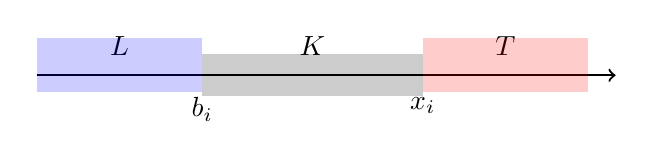
\begin{tikzpicture}[scale=7]
		\draw[->, thick] (0,0) -- (1.05,0);
		\foreach \x/\xtext in {0/,0.3/$b_i$,0.7/$x_i$,1/}
		\draw (\x,-0.65pt) node[below] {\xtext};

		\draw (0.15,0.5pt) node[above] {$L$};
		\draw (0.5,0.5pt) node[above] {$K$};
		\draw (0.85,0.5pt) node[above] {$T$};
		% \draw[-, ultra thick, blue] (0,0) -- (0.01,0);
		% \draw[-, ultra thick, blue] (0.19,0) -- (0.2,0);
		\fill[opacity = 0.2, blue] (0,-0.2ex) -- (0.3, -0.2ex) -- (0.3, 0.45ex) -- (0,0.45ex) -- cycle;
		\fill[opacity = 0.2, red] (0.7,-0.2ex) -- (1, -0.2ex) -- (1, 0.45ex) -- (0.7,0.45ex) -- cycle;
		\fill[opacity = 0.2, black] (0.3,-0.25ex) -- (0.7, -0.25ex) -- (0.7, 0.25ex) -- (0.3,0.25ex) -- cycle;
		% \draw (-0.25,0) node {$x=1$};
	\end{tikzpicture}
\end{center}

Existen tres posibilidades:

\begin{enumerate}
	\setlength{\itemsep}{0pt}
	\setlength{\parskip}{0pt}
	\setlength{\parsep}{0pt}
	\item El jugador $ i $ tiene la puja más grande, por lo tanto gana y paga $ b_j^* < b_i $ para $ j \neq i $. Esto corresponde a la situación en donde $ b_j^*, j\neq i $ está en la región $ L $. Suponiendo que en vez de $ b_i < x_i $ puja $ b_i = x_i $, de todas formas ganaría y, crucial, \textit{obtendría la misma utilidad}.
	\item El jugador $ j $ puja $ b_j^* > x_i $, por lo que $ i $ pierde (región $ T $). Aún así, $ i $ perdería incluso pujando $ b_i = x_i $.
	\item El jugador $ j $ puja $ b_i < b_j ^* <x_i $, en cuyo caso cae en la región $ K $, y el jugador $ i $ pierde, pero ganaría si pujara $ b_i = x_i $ y recibiría \[ u_i(b_i=x_i, b_j^*)=x_i - b_j^*\]
	      En este caso, pujar su valuación es estrictamente mejor que $ b_i < x_i $.
\end{enumerate}

Claramente, $ b_i = x_i $ dominante débilmente cualquier cantidad menorporque dicha estrategia \textit{nunca} es peor, y a veces es mejor. Similarmente, $ b_i > x_i $ es una estrategia débilmente denominada por $ b_i=x_i $ por las mismas razones, aunque en este caso, su utilidad no sería de 0, sino negativa.

Además de lo anterior, si las valuaciones son privadas, en subasta al segundo precio los jugadores no se preocupan por la distribución de probabilidad de los competidores.

Por último, el resultado de la subasta al segundo precio es \textit{Pareto óptima}\footnote{
	Una estrategia es Pareto-óptima si no empeora la situación de nadie más pero mejora la de un jugador. Es decir, $ u_i(s_i) \geq ui(s_i') $ para todos los $ i $, y $ u_i(s_i) > ui(s_i') $ para \textit{al menos} un $ i $.
}. La persona que más valora el bien es la que lo obtiene.

% \begin{tikzpicture}[>=stealth']

%   \begin{scope}[scale = 2]

%     \def\zval{1.65}

%     \draw[|-|, thick] (-\zval, 1) -- (\zval, 1);
%     \draw[fill = green] (0, 1) circle (1pt);
%     \node[below = 1ex] at (0, 1) {$\overline{y}$};
%     % \node[below] at (-\zval, 1) {$\overline{y} - \textcolor{cyan}{z_{\alpha/2}}\cdot \sigma/\sqrt{n}$};
%     % \node[below] at (\zval, 1) {$\overline{y} + \textcolor{orange}{z_{\alpha/2}}\cdot \sigma/\sqrt{n}$};

%     \draw [yshift = 1ex, decorate, decoration = {brace, amplitude = 5pt}] (-\zval, 1) -- (0, 1)
%       node [black, midway, yshift = 1.5em] {$e = z_{\alpha/2}\cdot \sigma/\sqrt{n}$};

%     \draw [yshift = 1ex, decorate, decoration = {brace, amplitude = 5pt}] (-\zval, 1.5) -- (\zval, 1.5)
%       node [black, midway, yshift = 1.5em] {$2e$};

%   \end{scope}

% \end{tikzpicture}%

\section*{Recordatorio}
\subsection*{Tratamiento sistemático de los juegos con información incompleta}
\textbf{En un juego con información incompleta} se tienen que seguir los siguientes pasos e indicaciones para obtener el ENB.

\begin{enumerate}
	\setlength{\itemsep}{0pt}
	\setlength{\parskip}{0pt}
	\setlength{\parsep}{0pt}
	\item Los tipos (qué información es privada, y para qué jugador es privada).
	\item La distribución de probabilidad de los tipos.
	\item Si el juego es de información asimétrica (como el mercado de coches usados, o como en la competencia de Cournot ), o simétrica (como en las subastas, donde todos los jugadores tienen información privada).
	\item La función de utilidad para cada jugador.
	      \begin{itemize}
		      \item Si el juego es de información asimétrica, como en Cournot, los jugadores tendrán diferente función de utilidad: el jugador con más de un tipo, tendrá tantas funciones de utilidad como tipos; el jugador con un solo tipo solo tendrá una función de utilidad, pero promediada a través de los tipos de (los) otro (s) jugadores (su utilidad esperada será la suma de la utilidad cuando el otro jugador juega un tipo, multiplicada por la probabilidad de ese tipo, más la suma de la utilidad cuando el otro jugador juega su otro tipo, multiplicada por la probabilidad de ese otro tipo, etc.).
		      \item Si el juego es de información simétrica como en la subasta de sobre cerrado al primer precio, y si los jugadores usan estrategias simétricas (por ejemplo, si usan una fracción $ a $ común a todos los jugadores) la solución será la misma para todos los jugadores. (De hecho, en una subasta de sobre cerrado al primer precio, la solución de la puja óptima depende de la cantidad de jugadores, no de lo que los otros pujen).
	      \end{itemize}
	\item Maximizar la utilidad esperada de los juagdores. De nuevo, la utilidad esperada será una suma de utilidad multiplicada por la probabilidad de la ocurrencia del evento. Por ejemplo, en un duopolio de Cournot, la utilidad esperada del jugador con un solo tipo es la suma de dos utilidades (una cuando el otro jugador tiene, por ejemplo, costo alto; otra cuando el otro jugador tiene costo bajo) multiplicada por dos probabilidad (respectivamente, la probabilidad de que el otro jugador tenga costo bajo y la probabilidad de que el otro jugador tenga costo bajo).
\end{enumerate}

\end{document}